% Use this if you generate the presentation itself.
\documentclass[%
final,
xcolor = table,
usenames,
dvipsnames,
table,
aspectratio = 169]{beamer}

% Use this documentclass line for generating the handout
% \documentclass[%
% final,
% xcolor = table,
% usenames,
% dvipsnames,
% table,
% hadout,
% draft,
% aspectratio = 169,
% ]{beamer}

\usepackage{appendixnumberbeamer}

% minted load packages: keyval, ifthen, etoolbox, kvoptions, calc, xstring,
% fancyvrb, ifplatform, xcolor, float, pdftexcmds, lineno
\usepackage[outputdir = ../.latex-cache]{minted} % minted above polyglossia, because errors
\usemintedstyle{perldoc}

%% Two version of compilers (pdflatex, xelatex)
\usepackage{ifxetex}
%% XeTeX
\ifxetex
    \usepackage{polyglossia} % Multilanguages

    \usepackage{xunicode} % Generate Unicode chars from accented glyphs.
    \usepackage{xltxtra} % "Extras" for LaTeX users of XeTeX.

    % Support of russian language (hyphenation, styles, etc.)
    \setmainlanguage{english} % default language --- English
    \setotherlanguage{russian} % additional language --- Russian

    %% Fonts
    % \defaultfontfeatures{Ligatures=TeX,Mapping=tex-text}
    % \setmainfont{CMU Serif}
    % \setsansfont{CMU Sans Serif}
    % \setmainfont{Droid Serif}
    % \newfontfamily\cyrillicfont{Fira Sans Light}[BoldFont={Fira Sans}]%
    % \setsansfont{Droid Sans}
    % \newfontfamily\cyrillicfontsf{Droid Sans}
    % \setmonofont{CMU Typewriter Text}
    \setmonofont{Anonymous Pro}
    % \newfontfamily\cyrillicfonttt{Anonymous Pro}
\else
    \usepackage[T2A]{fontenc}
    \usepackage[utf8]{inputenc}
    \usepackage{lmodern}
\fi

\usepackage{graphicx} % Images
\usepackage{pdfpages} % PDFs
\usepackage{pgfpages} % Two screens

\usepackage{multirow} % Multirows in tables

% Set path for graphics
\graphicspath{{../images/}}

%% Vector graphics
\usepackage{tikz}

\usetikzlibrary{arrows.meta,
  automata,
  backgrounds,
  calc,
  decorations.markings,
  decorations.pathmorphing,
  fit,
  graphs,
  matrix,
  positioning,
  shapes.geometric,
  shapes.misc,
  shapes.multipart,
  tikzmark,
}

% ==============================================================================

\mode<presentation>
{

  %% Theme settings
  \usetheme{dsec}
  \dsecset{progressbar = frametitle}
  \dsecset{subsectionpage = progressbar}

  %% Notes settings
  % \setbeameroption{hide notes}
  % \setbeameroption{show notes}
  % \setbeameroption{show notes on second screen = right}
  % \setbeameroption{show only notes}

  % Style of notes
  \setbeamertemplate{note page}[plain]
}

%% Fix bug with beamer + xelatex + notes
% https://tex.stackexchange.com/questions/232168/normal-text-is-invisible-when-using-beamer-with-notes-and-xelatex
\makeatletter
\def\beamer@framenotesbegin{% at beginning of slide
     \usebeamercolor[fg]{normal text}
      \gdef\beamer@noteitems{}%
      \gdef\beamer@notes{}%
}
\makeatother

% ==============================================================================

\title{Rust and what's this thing for}

\author{Abc Xyz\\
@dura\_lex}
\institute{
\includegraphics[height = 2cm]{rust_logo.pdf}}
\titlegraphic{
\includegraphics[height = 0.9cm]{logo.pdf}}

\date{}
\subject{Rust}

% ==============================================================================

\begin{document}

\maketitle
\note{

  Хочу рассказать предисловие.

  Когда я устраивался в DSec, то я позиционировался на позицию реверс-инженера и
  программиста. Моим заданием на программиста было написание загрузчика ELF
  файлов с проверкой цифровой подписи. В связи с тем, что к тому времени я уже
  писал в production на Rust, своё решение я написал с 0 на Rust. Когда я
  проходил собеседование, то узнал, что нужно было взять Linux загрузчик на C и
  модифицировать его. В общем, на программиста меня не взяли.

  В первый же день моей работы мы с Ромой завели разговор о Rust, и Рома сказал
  сделать мне доклад о Rust в нерабочее время. Честно сказать, тогда я весьма
  опешил, потому что на моей прошлой работе не было никаких докладов, да и в
  нерабочее время заниматься работой я не хотел.

  К чему я это? А к тому, что доклад по Rust я начал вынашивать с момента моего
  устройства на работу, готовить начал с прошлого года.

}

%% Set theme colors
\tikzset{%
  text = dBlack,%
  % draw = White,%
}

% ------------------------------------------------------------------------------

\begin{frame}{Agenda}
  \setbeamertemplate{section in toc}[sections numbered]%
  \begin{columns}
    \begin{column}{.5\textwidth}
      \tableofcontents[hideothersubsections, sections = {1-4}]
    \end{column}
    \begin{column}{.5\textwidth}
      \tableofcontents[hideothersubsections, sections = {5-8}]
    \end{column}
  \end{columns}
\end{frame}

% ------------------------------------------------------------------------------

\section{Foreword}
\begin{frame}{Motivation}

  \center%
  \includegraphics<1>[width = 0.9\textwidth]{c_p_p_die.jpg}
  \includegraphics<2>[height = 0.9\textheight]{rust_evangelism.png}

  \note<1>{

    В последнее время \textbf{всё чаще} в IT новостях можно услышать, что был
    разработан тот или иной \textbf{проект на Rust}, будь то Web (WebAssembly)
    или Embedded (TrustZone, IoT) или GameDev или консольная утилита или новая
    ОС или файловая система или кодек или декодировщик и т. д.

    Интерес к языку среди программистов растёт всё больше и больше. Вот уже и
    \textbf{среди безопасников интерес также подогревается}, не смотря на то,
    что многие относятся скептически. Я даже \textbf{в исследовательском центре}
    всё чаще сталкиваюсь с проектами на Rust: при изучении ChromeBook (система
    виртуализации, песочница), блокчейн проектов (Rust здесь практически
    лидирует), изучение новых фаззеров (на Rust), в IoT устройствах.

  }
      

  \note<2>{

    Я отчасти Rust евангелист (в принципе как и евангелист Linux и KISS
    принципа), поэтому буду призывать попробовать данный язык по возможности.
    Статистика показывает, что \textbf{люди, которые перешагнули определённый
      порог} при изучении, \textbf{получают удовольствие} от того, что
    разрабатывают на Rust.

    Мне интересны языки программирования, поэтому я знаю, что существует ещё
    множество других интересных и полезных языков (Racket, Haskell, Ada, OCaml,
    SPARK, Coq, Nim и др.), поэтому выбирайте язык исходя из задачи, а не
    задачу, исходя из известного вам языка.

    В своём докладе я сделаю упор на сам язык, а не на его аудит, т. к. на
    сколько мне известно, до сих пор небольшой процент людей нашей компании
    знаком с данным языком. Это недоразумение я и хочу исправить.
      
  }
\end{frame}

\begin{frame}{Experience}

  \begin{columns}
    \begin{column}{0.6\textwidth}
      \begin{itemize}
      \item Since 1.0.0
      \item Scope (by time)
        \begin{itemize}
        \item Bindings (FFI --- foreign function interface)
        \item Analyzers
        \item CLI (TUI) tools for PC and IoT
        \item GUI for fun
        \item Libraries
        \item RE
        \end{itemize}
      \item Nim, Crystal, Zig, Pony
      \end{itemize}
    \end{column}
    \begin{column}{0.4\textwidth}
      
\includegraphics[width = 0.9\textwidth]{rust_ussr.png}
    \end{column}
  \end{columns}

  \note{

    \textbf{Начал} более-менее изучать Rust в то время, когда его версия стала
    \textbf{стабильной}, до этого только смотрел примеры кода. В то время
    занимался «железом», поэтому интересно было изучать такие языки, как C, Ada
    (Spark), Rust.

    \textbf{Начинал} с того, с чего обычно не начинают --- с байндингов (FFI)
    для нужных мне инструментов. Затем стал разрабатывать \textbf{анализатор
      НДВ}. Между делом для себя писал консольные тулы (\textbf{слез с Python}).
    Затем помогал в разработке различных библиотек.

    Знаком и писал на других \textbf{новых языках}, также писал и немного знаю
    концепции \textbf{C, Ada, Haskell, Lisp, Python}.

  }
\end{frame}

\begin{frame}{I'm not true programmer}
  \center
  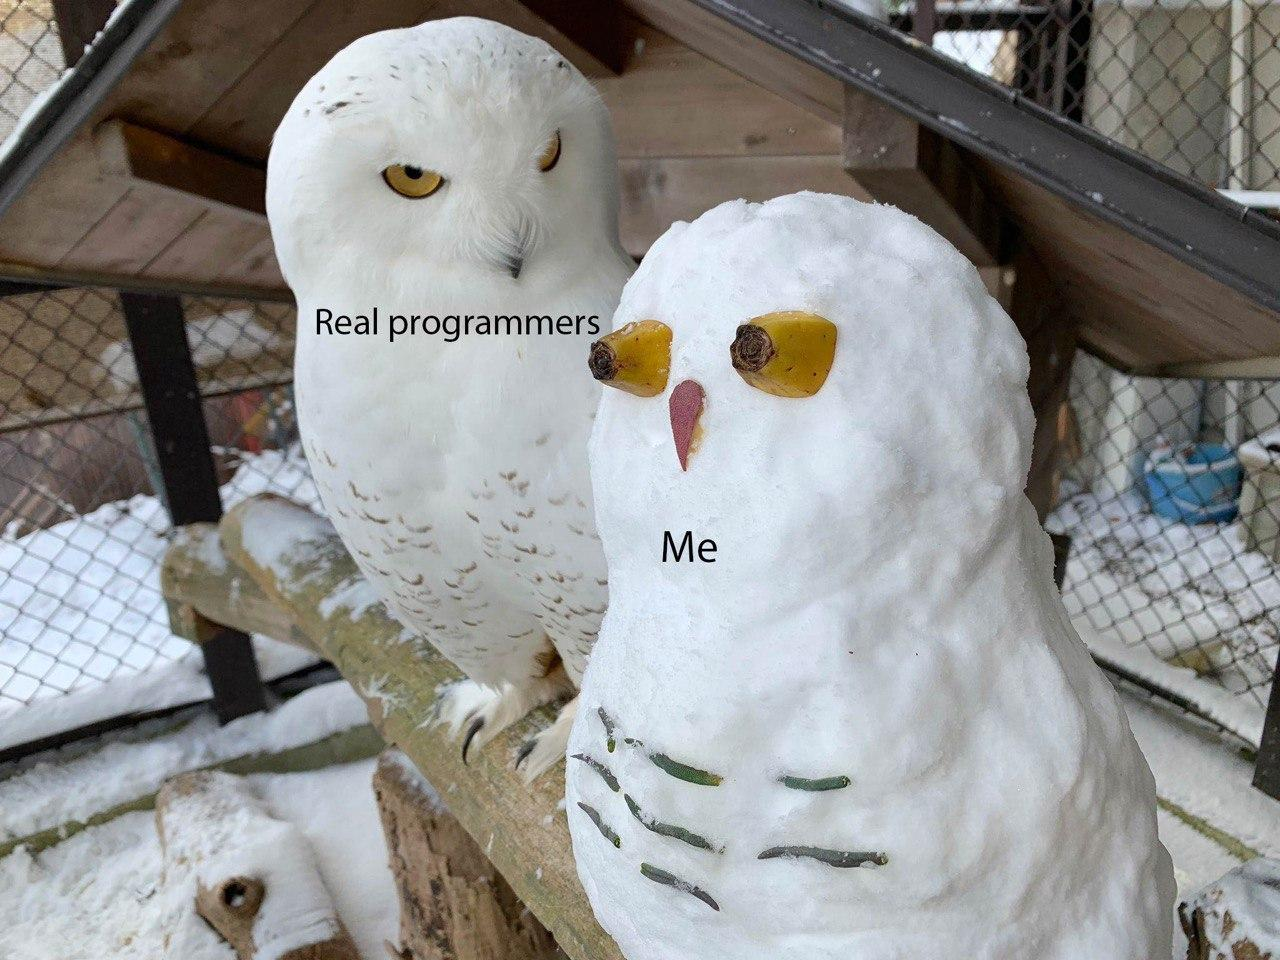
\includegraphics[width = 0.65\textwidth]{real_programmers}

  \note {

    Я не программист и не реверсер. На программиста \textbf{не учился}, читал
    книги, поэтому много \textbf{пробелов в матчасти}.

    Буду рассказывать, исходя только из \textbf{собственного опыта}, моё мнение
    может не совпадать с мнением многих других людей (постоянные холивары).

    \textbf{Я не буду учить вас Rust}, я просто расскажу основные концепции и
    фишки.

  }
\end{frame}

% ------------------------------------------------------------------------------

\section{What is Rust?}
\begin{frame}{\insertsection}

  \textit{``\textbf{Rust} is a multi-paradigm systems programming language
    focused on safety, especially safe concurrency''.}
  \\[5pt]
  \rightline{{---
      \href{https://en.wikipedia.org/wiki/Rust_(programming_language)}{Wikipedia}}}

  \note{

    Википедия говорит, что Rust --- это мультипарадигменный системный язык
    программирования, нацеленный на безопасность, особенно на безопасность при
    параллелизме.

  }
\end{frame}

\begin{frame}{\insertsection}

  \textit{``\textbf{Rust} is a systems programming language that \textbf{runs
      blazingly fast}, \textbf{prevents nearly all segfaults}, and
    \textbf{guarantees thread safety}''.}
  \\[5pt]
  \rightline{{--- www.rust-lang.org (2015)}}

  \note{

    На официальном сайте \textbf{раньше} подчёркивались такие черты языка, как
    \textbf{быстрая скорость выполнения}, \textbf{предотвращение ошибок
      сегментации} и \textbf{гарантия безопасности при работе с потоками}.

  }
\end{frame}

\begin{frame}{\insertsection}

  \textit{``Empowering everyone to build reliable and efficient software''.}
  \\[5pt]
  \rightline{{--- \href{https://www.rust-lang.org/}{www.rust-lang.org}}}

  \note{

    На данный момент язык находится в процессе расширения и смены ориентации,
    отсюда появляются \textbf{другие цели}.

  }
\end{frame}

\subsection{Quick facts about Rust}
\begin{frame}{\insertsubsection}

  \begin{itemize}
  \item Started by Mozilla (sponsorship \& support) employee Graydon Hoare
  \item First announced by Mozilla in 2010
  \item Community driven development
  \item 88,281 commits on GitHub
  \item First stable release: 1.0 in May 2015
  \item Latest stable release: 1.32
  \end{itemize}

  \note{

    \begin{itemize}
    \item Был написан на \textbf{OCaml}
    \item Mozilla поддержала инициативу Грейдона для написания своего движка для
      браузера --- \textbf{Servo}
    \item Любой может влиться в разработку, сделать своё предложение в виде
      \textbf{RFC --- Request for Comments}, в отличие от C++ и других
    \item Является одним из самых \textbf{популярных репозиториев} на GitHub,
      \textbf{самым любимым языком} на StackOverflow
    \item Недавно произошло радикальное изменение языка (\textbf{2018 edition}),
      но обратная совместимость от этого не пострадала
    \end{itemize}

  }
\end{frame}


\subsection{Why Rust?}
\begin{frame}{\insertsubsection}
  \begin{columns}
    \begin{column}{0.4\textwidth}
      
\includegraphics[height = 0.8\textheight]{rust_lang.jpg}
    \end{column}
    \begin{column}{0.6\textwidth}
      \begin{itemize}
      \item Performance
        \begin{itemize}
        \item Fast, memory-efficient
        \item No runtime or garbage collector
        \item Zero-cost abstractions
        \end{itemize}
      \item Reliability
        \begin{itemize}
        \item Rich type system
        \item Ownership model
        \end{itemize}
      \item Productivity
        \begin{itemize}
        \item Documentation
        \item Friendly compiler
        \item Top-notch tooling
        \end{itemize}
      \end{itemize}
    \end{column}
  \end{columns}

  \note{

    Какие характерные черты данного языка можно выделить?

    \begin{itemize}
    \item Быстрый за счёт \textbf{нулевой стоимости абстракций}, без GC, поэтому
      можно \textbf{встраивать в другие языки}, в \textbf{критические сервисы},
      запускать \textbf{на встраиваемых системах}.
    \item Богатая система типов и модель владения, отсюда --- \textbf{безопасная
        работа} с памятью и потоками, многие ошибки отлавливаются \textbf{во
        время компилирования}.
    \item Благодаря \textbf{дружелюбному сообществу} и \textbf{open-source
        разработке} у Rust много преимуществ.
    \end{itemize}

  }
\end{frame}


% ------------------------------------------------------------------------------

\section{(Un)safe}

\subsection{Control vs Safety}
\begin{frame}{\insertsubsection}
  \center
  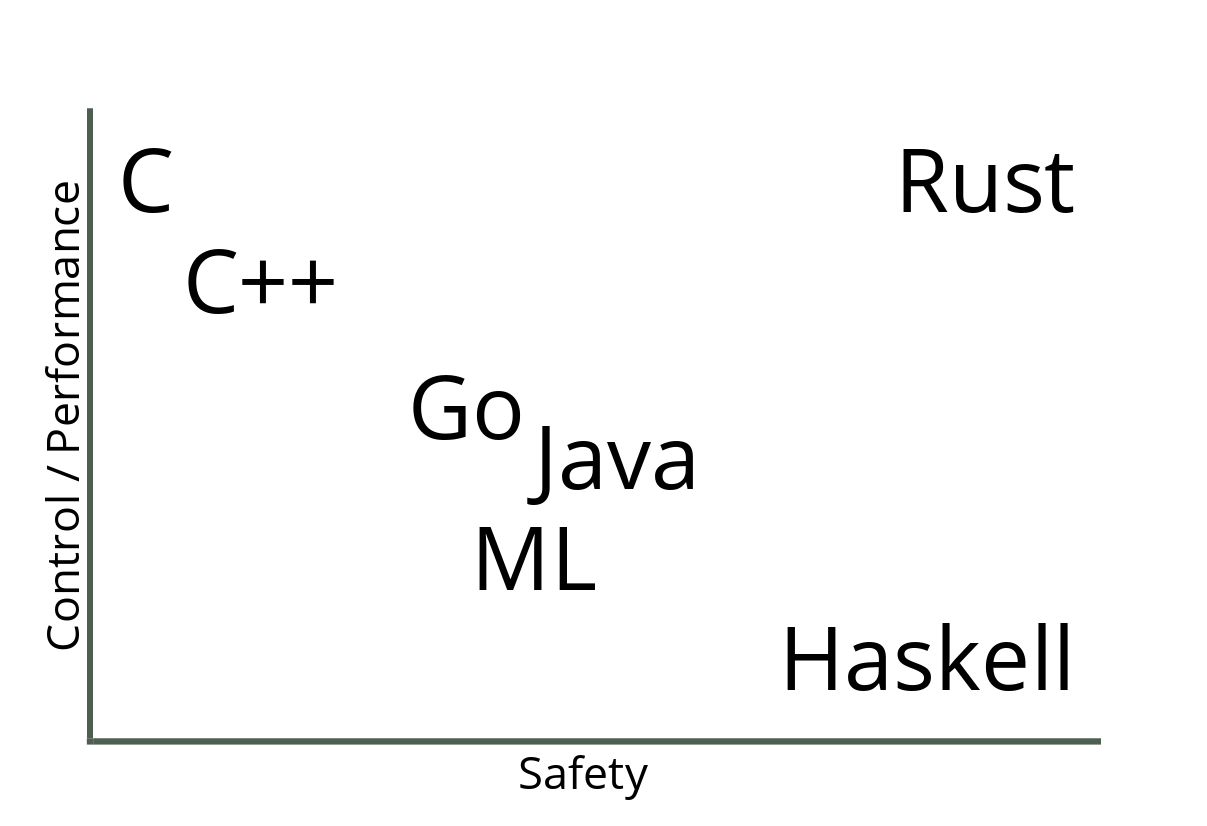
\includegraphics[height = 0.85\textheight]{control_safety.png}

  \note {

    Есть низкоуровневые языки, которые позволяют контролировать всё и вся,
    жертвуя при этом безопасностью. Есть высокоуровневые языки, которые не
    менее производительны, зато более безопасные. Также есть языки, с богатой
    системой типов, которые отличаются своей безопасностью, но не
    производительностью (IDRIS). А есть Rust!

  }
\end{frame}

\subsection{What's wrong with systems languages?}
\begin{frame}{\insertsubsection}

  \begin{itemize}
  \item It's difficult to write secure code
  \item It's very difficult to write multithreaded code
  \end{itemize}

  Rust?

  \note{

    Программируя на системных ЯП, сталкиваешься с определёнными проблемами (на
    слайде). Rust был \textbf{задуман} как раз \textbf{для решения этих
      проблем}. Конечно же, это \textbf{не серебряная пуля}.

  }
\end{frame}


\subsection{Problems}
\begin{frame}{\insertsubsection}

  \begin{columns}
    \begin{column}{0.6\textwidth}
    Memory corruption
    \begin{itemize}
    \item Using uninitialized memory
    \item Using non-owned memory (null pointer, dangling pointer dereference,
      out of bounds error)
    \item Using memory beyond the memory that was allocated (buffer overflow)
    \item Faulty heap memory management (memory leaks, freeing non-heap or
      un-allocated memory)
    \end{itemize}
  \end{column}
  \begin{column}{0.4\textwidth}
    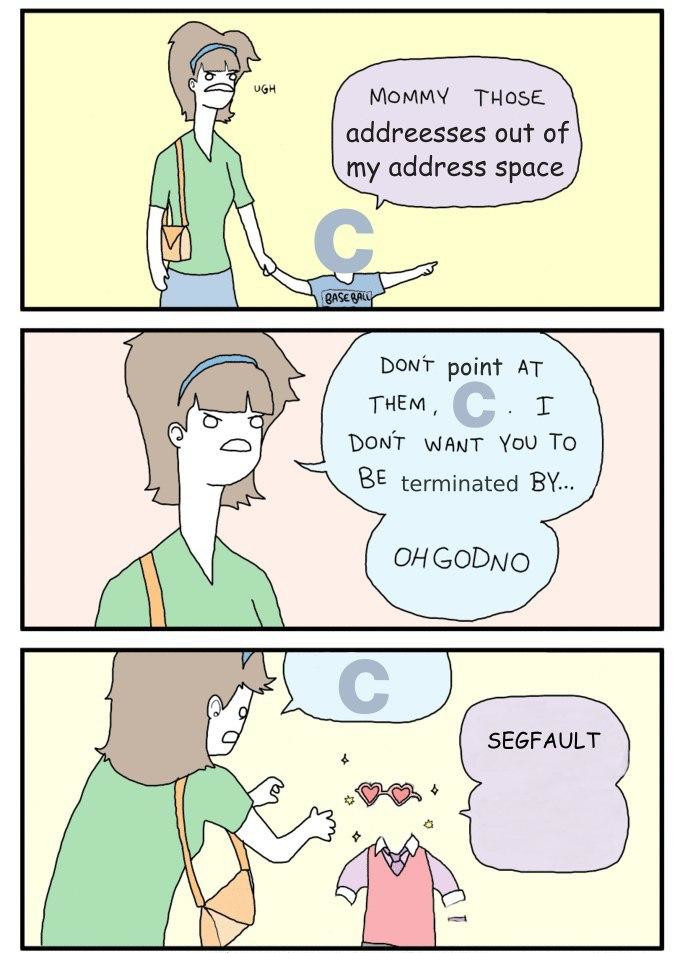
\includegraphics[width = 0.8\textwidth]{c_out_of_space.jpg}
  \end{column}
\end{columns}

  \note{

    В системных (и не только: Java, C\#) языках \textbf{существуют проблемы с
      безопасностью при работе с памятью}. Rust нацелен на решение этих самых
    проблем.

    Примеры проблем:

    \begin{itemize}
    \item использование не инициализированной памяти;
    \item использование не принадлежащей программе памяти;
    \item использование памяти за пределами выделенной;
    \item ошибки управления памятью на куче.
    \end{itemize}
    
  }
\end{frame}


\subsection{Ownership and Borrowing}
{

  \setbeamercolor{background canvas}{bg=}%
  \includepdf[pages = 1]{o_and_b.pdf}%

  \note {

    Для того, чтобы понять, \textbf{почему Rust} считается безопасным языком,
    нужно понимать, \textbf{как он работает}, какие концепции используются.

    Мне было лень, поэтому я взял хорошо оформленные и понятные слайды
    презентации Николаса Матсакиса (один из главных разработчиков Rust), за что
    ему большое спасибо.

  }

}

{

  \setbeamercolor{background canvas}{bg=}%
  \includepdf[pages = 38]{o_and_b.pdf}%

  \note {

    \textbf{Владение и заимствование} --- вот одни из главных концепций ЯП Rust.

    На следующих слайдах я расскажу, что это такое.

  }

}

{

  \setbeamercolor{background canvas}{bg=}%
  \includepdf[pages = 39]{o_and_b.pdf}%

  \note {

    И так, концепция \textbf{владения}.

    У нас есть книга, мы ею \textbf{владеем}.

  }

}

{

  \setbeamercolor{background canvas}{bg=}%
  \includepdf[pages = 40]{o_and_b.pdf}%

  \note {

    Как только \textbf{мы передаём} книгу, мы \textbf{перестаём ей владеть}. У
    книги появляется новый хозяин.

  }

}

{

  \setbeamercolor{background canvas}{bg=}%
  \includepdf[pages = 41]{o_and_b.pdf}%

  \note {

    Рассмотрим на примере кода.

    У нас есть переменная \texttt{name} (\textbf{наша книга}) типа
    \texttt{String}.

  }

}

{

  \setbeamercolor{background canvas}{bg=}%
  \includepdf[pages = 42]{o_and_b.pdf}%

  \note {

    Также у нас есть функция \texttt{helper} --- будущий хозяин нашей строки
    (книги). Что же происходит при вызове функции?

  }

}

{

  \setbeamercolor{background canvas}{bg=}%
  \includepdf[pages = 43]{o_and_b.pdf}%

  \note {

    Посмотрим на определение функции \texttt{helper} --- в качестве параметра
    она принимает объект с типом \texttt{String}. Она принимает \textbf{не
      ссылку} и \textbf{не само значение}, а именно возможность владения данным
    \textbf{объектом}, если можно так сказать.

  }

}

{

  \setbeamercolor{background canvas}{bg=}%
  \includepdf[pages = 44]{o_and_b.pdf}%

  \note {

    Возвращаемся обратно, \textbf{вызываем функцию}.

  }

}

{

  \setbeamercolor{background canvas}{bg=}%
  \includepdf[pages = 45]{o_and_b.pdf}%

  \note {

    При вызове функции у нас \textbf{происходит смена владельца} нашей книги.

  }

}

{

  \setbeamercolor{background canvas}{bg=}%
  \includepdf[pages = 46-47]{o_and_b.pdf}%

  \note {

    После того, как \textbf{функция отработала} --- она, то бишь хозяин,
    \textbf{исчезает}.

  }

}

{

  \setbeamercolor{background canvas}{bg=}%
  \includepdf[pages = 48]{o_and_b.pdf}%

  \note {

    А если \textbf{исчезает хозяин}, то вместе и \textbf{с ним объект}, которым
    он владел. Это называется \textbf{RAII} (Resource acquisition is
    initialization) --- \textbf{получение ресурса есть инициализация}.

  }

}

{

  \setbeamercolor{background canvas}{bg=}%
  \includepdf[pages = 49]{o_and_b.pdf}%

  \note {

    Если мы попытаемся \textbf{ещё раз вызвать функцию}, которая в качестве
    аргумента принимает объект, которого \textbf{у нас уже нет}, т. к. мы его
    уже отдали, \textbf{что же тогда произойдёт}?

  }

}

{

  \setbeamercolor{background canvas}{bg=}%
  \includepdf[pages = 50]{o_and_b.pdf}%

  \note {

    Правильно, \textbf{ошибка} --- использование уже перемещённого значения.

  }

}

{

  \setbeamercolor{background canvas}{bg=}%
  \includepdf[pages = 51]{o_and_b.pdf}%

  \note {

    Посмотрим как данная концепция (или \textbf{её подобие}) реализована в
    других языках.

    У нас также есть объект, но типа \texttt{Vector} (что по сути также может
    быть строкой, вектором символов).

  }

}

{

  \setbeamercolor{background canvas}{bg=}%
  \includepdf[pages = 52]{o_and_b.pdf}%

  \note {

    У нас есть функция, которая также в качестве параметра принимает объект типа
    \texttt{Vector}.

  }

}

{

  \setbeamercolor{background canvas}{bg=}%
  \includepdf[pages = 53]{o_and_b.pdf}%

  \note {

    Но в данном случае параметр функции передаётся \textbf{в качестве ссылки}.

  }

}

{

  \setbeamercolor{background canvas}{bg=}%
  \includepdf[pages = 54]{o_and_b.pdf}%

  \note {

    Снова возвращаемся и вызываем нашу функцию.

  }

}

{

  \setbeamercolor{background canvas}{bg=}%
  \includepdf[pages = 56]{o_and_b.pdf}%

  \note {

    В \textbf{Java} при вызове функции у нас оказывается два хозяина одного
    объекта.

  }

}

{

  \setbeamercolor{background canvas}{bg=}%
  \includepdf[pages = 57]{o_and_b.pdf}%

  \note {

    Хорошо. Продолжаем выполнение функции.

  }

}

{

  \setbeamercolor{background canvas}{bg=}%
  \includepdf[pages = 58]{o_and_b.pdf}%

  \note {

    Функция закончила своё выполнение.

  }

}

{

  \setbeamercolor{background canvas}{bg=}%
  \includepdf[pages = 59]{o_and_b.pdf}%

  \note {

    Функция исчезает, как и в Rust. Но \textbf{что же происходит с объектом}?

  }

}

{

  \setbeamercolor{background canvas}{bg=}%
  \includepdf[pages = 60]{o_and_b.pdf}%

  \note {

    Объект никуда не пропадает, он \textbf{остаётся у своего первоначального
      хозяина}.

    Также \textbf{возможен повторный вызов} функции \texttt{helper}.

  }

}

{

  \setbeamercolor{background canvas}{bg=}%
  \includepdf[pages = 61]{o_and_b.pdf}%

  \note {

    Главная функция заканчивает свою работу и также исчезает.

  }

}

{

  \setbeamercolor{background canvas}{bg=}%
  \includepdf[pages = 62]{o_and_b.pdf}%

  \note {

    При этом \textbf{созданный функцией объект остаётся}. \textbf{Для чего это
      нужно?}

  }

}

{

  \setbeamercolor{background canvas}{bg=}%
  \includepdf[pages = 63]{o_and_b.pdf}%

  \note {

    Представим, что функция \texttt{helper} внутри себя создаёт поток.

  }

}

{

  \setbeamercolor{background canvas}{bg=}%
  \includepdf[pages = 64]{o_and_b.pdf}%

  \note {

    Тогда хозяином объекта, даже после исчезновения главной функции, будет
    функция \texttt{helper}.

  }

}

{

  \setbeamercolor{background canvas}{bg=}%
  \includepdf[pages = 65]{o_and_b.pdf}%

  \note {

    Когда поток закончит свою работу, то текущий хозяин объекта также перестанет
    существовать.

  }

}

{

  \setbeamercolor{background canvas}{bg=}%
  \includepdf[pages = 66]{o_and_b.pdf}%

  \note {

    Ну а сборщик мусора сделает своё дело...

  }

}

{

  \setbeamercolor{background canvas}{bg=}%
  \includepdf[pages = 67]{o_and_b.pdf}%

  \note {

    ... и удалит уже никому ненужный объект.

  }

}

{

  \setbeamercolor{background canvas}{bg=}%
  \includepdf[pages = 68]{o_and_b.pdf}%

  \note {

    Рассмотрим одну интересную особенность в Rust при передаче права владения
    объектом, а именно концепцию \textbf{клонирования}.

  }

}

{

  \setbeamercolor{background canvas}{bg=}%
  \includepdf[pages = 69]{o_and_b.pdf}%

  \note {

    Всё также вызываем нашу функцию \texttt{helper}.

  }

}

{

  \setbeamercolor{background canvas}{bg=}%
  \includepdf[pages = 70]{o_and_b.pdf}%

  \note {

    Но при передаче прав владения объектом \textbf{мы делаем клон} этого самого
    объекта!

  }

}

{

  \setbeamercolor{background canvas}{bg=}%
  \includepdf[pages = 72]{o_and_b.pdf}%

  \note {

    То есть в функцию мы отдаём не сам объект, а его клон.

  }

}

{

  \setbeamercolor{background canvas}{bg=}%
  \includepdf[pages = 73]{o_and_b.pdf}%

  \note {

    Вызываем функцию.

  }

}

{

  \setbeamercolor{background canvas}{bg=}%
  \includepdf[pages = 74]{o_and_b.pdf}%

  \note {

    После того, как функция отработает, \textbf{она исчезает} и исчезает
    аргумент, как было показано ранее, но при этом \textbf{исчезает клон
      объекта}, а не сам объект!

  }

}

{

  \setbeamercolor{background canvas}{bg=}%
  \includepdf[pages = 75]{o_and_b.pdf}%

  \note {

    После этого мы повторно можем вызвать функцию \texttt{helper}, но передать
    уже оригинальный объект.

  }

}

{

  \setbeamercolor{background canvas}{bg=}%
  \includepdf[pages = 76]{o_and_b.pdf}%

  \note {

    В этом случае, мы, конечно же, его уже теряем.

  }

}

{

  \setbeamercolor{background canvas}{bg=}%
  \includepdf[pages = 77]{o_and_b.pdf}%

  \note {

    Есть один небольшой нюанс в концепции клонирования --- \textbf{копирование}
    или по-другому \textbf{авто-клонирование}.

  }

}

{

  \setbeamercolor{background canvas}{bg=}%
  \includepdf[pages = 78]{o_and_b.pdf}%

  \note {

    Если тип объекта \textbf{обладает свойством копирования (реализован типаж)},
    то при передаче прав владения \textbf{клонирование происходит
      автоматически}.

  }

}

{

  \setbeamercolor{background canvas}{bg=}%
  \includepdf[pages = 79]{o_and_b.pdf}%

  \note {

    Вызовем функцию \texttt{helper} в первый раз, передав при этом целочисленный
    тип \texttt{i32}, который обладает свойством \texttt{Copy}.

  }

}

{

  \setbeamercolor{background canvas}{bg=}%
  \includepdf[pages = 80]{o_and_b.pdf}%

  \note {

    Произойдёт автоматическое клонирование при передаче прав владения.

  }

}

{

  \setbeamercolor{background canvas}{bg=}%
  \includepdf[pages = 81]{o_and_b.pdf}%

  \note {

    После исполнения функции объект исчезает.

  }

}

{

  \setbeamercolor{background canvas}{bg=}%
  \includepdf[pages = 82]{o_and_b.pdf}%

  \note {

    При втором вызове функции \texttt{helper} происходит то же самое, то есть
    \textbf{объект остаётся у функции-создателя}.

  }

}

{

  \setbeamercolor{background canvas}{bg=}%
  \includepdf[pages = 83]{o_and_b.pdf}%

  \note {

    Подытожим.

    У нас есть \textbf{некопируемые объекты}, при передаче прав владения
    которых, \textbf{передаётся сам объект}.

    У нас есть \textbf{объекты с возможностью клонирования}, для которых мы
    вручную можем задать, чтобы передаче прав владения \textbf{создавался клон
      объекта}.

    И у нас есть объекты, которые имеют \textbf{свойство \texttt{Copy}}. Данные
    объекты \textbf{прозрачно для разработчика копируются} при передаче в
    качестве аргумента.

  }

}
{

  \setbeamercolor{background canvas}{bg=}%
  \includepdf[pages = 85]{o_and_b.pdf}%

  \note {

    Концепция \textbf{заимствования}.

    Разделяемые заимствования.

    У нас как всегда \textbf{есть книга дракона}.

  }

}

{

  \setbeamercolor{background canvas}{bg=}%
  \includepdf[pages = 86]{o_and_b.pdf}%

  \note {

    Мы \textbf{отдаём} эту книгу, но \textbf{с условием, что нам её вернут}.

  }

}

{

  \setbeamercolor{background canvas}{bg=}%
  \includepdf[pages = 87]{o_and_b.pdf}%

  \note {

    \textbf{После того}, как нашу книгу \textbf{прочитали}, нам её
    \textbf{возвращают}.

    В отличие от передачи прав владения, мы даём книгу только \textbf{на время}.

  }

}

{

  \setbeamercolor{background canvas}{bg=}%
  \includepdf[pages = 88]{o_and_b.pdf}%

  \note {

    Теперь рассмотрим пример кода.

    У нас всё так же есть переменная \texttt{name} типа \texttt{String}.

  }

}

{

  \setbeamercolor{background canvas}{bg=}%
  \includepdf[pages = 90]{o_and_b.pdf}%

  \note {

    Обратите внимание, как поменялся тип параметра --- теперь передаётся не
    объект, а ссылка на объект, то бишь ссылка на переменную типа
    \texttt{String}.

  }

}

{

  \setbeamercolor{background canvas}{bg=}%
  \includepdf[pages = 92]{o_and_b.pdf}%

  \note {

    Чтобы передать нашу строку функции, \textbf{нам нужно получить ссылку},
    делаем это.

  }

}

{

  \setbeamercolor{background canvas}{bg=}%
  \includepdf[pages = 96]{o_and_b.pdf}%

  \note {

    Вызываем функцию \texttt{helper} и \textbf{передаём ей ссылку} на строку в
    качестве аргумента.

    Стоить заметить, что \textbf{ссылка на объект также остаётся у нас} в
    пользовании.

  }

}

{

  \setbeamercolor{background canvas}{bg=}%
  \includepdf[pages = 97]{o_and_b.pdf}%

  \note {

    Функция выполняется.

  }

}

{

  \setbeamercolor{background canvas}{bg=}%
  \includepdf[pages = 98]{o_and_b.pdf}%

  \note {

    Функция заканчивает своё выполнение.

  }

}

{

  \setbeamercolor{background canvas}{bg=}%
  \includepdf[pages = 99]{o_and_b.pdf}%

  \note {

    Функция исчезает, а с ней \textbf{исчезает и ссылка}.

  }

}

{

  \setbeamercolor{background canvas}{bg=}%
  \includepdf[pages = 100]{o_and_b.pdf}%

  \note {

    Мы снова можем вызвать функцию \texttt{helper}, передав ссылку на объект.

  }

}

{

  \setbeamercolor{background canvas}{bg=}%
  \includepdf[pages = 102]{o_and_b.pdf}%

  \note {

    Когда главная \textbf{функция прекращает своё выполнение}, то \textbf{и
      ссылка, и объект уничтожаются}.

  }

}

{

  \setbeamercolor{background canvas}{bg=}%
  \includepdf[pages = 103]{o_and_b.pdf}%

  \note {

    Стоит сказать, что в Rust \textbf{все объекты}, будь то значение или ссылки
    --- \textbf{неизменяемые} по умолчанию.

  }

}

{

  \setbeamercolor{background canvas}{bg=}%
  \includepdf[pages = 104]{o_and_b.pdf}%

  \note {

    Поэтому, если мы просто \textbf{читаем данные}, переданные нам по ссылке, то
    всё будет \textbf{хорошо}.

  }

}

{

  \setbeamercolor{background canvas}{bg=}%
  \includepdf[pages = 105]{o_and_b.pdf}%

  \note {

    А если попробуем \textbf{изменить} данные, то получим \textbf{ошибку}.

  }

}

{

  \setbeamercolor{background canvas}{bg=}%
  \includepdf[pages = 106]{o_and_b.pdf}%

  \note {

    Ошибку \textbf{компиляции}.

  }

}

{

  \setbeamercolor{background canvas}{bg=}%
  \includepdf[pages = 107]{o_and_b.pdf}%

  \note {

    На самом деле, данные \textbf{можно изменять}, но \textbf{только
      контролируемо}, об этом я не буду рассказывать подробно, считайте, что
    \textbf{по умолчанию всё неизменяемое}.

  }

}

{

  \setbeamercolor{background canvas}{bg=}%
  \includepdf[pages = 108]{o_and_b.pdf}%

  \note {

    Побольше рассмотрим ссылки.

  }

}

{

  \setbeamercolor{background canvas}{bg=}%
  \includepdf[pages = 109]{o_and_b.pdf}%

  \note {

    Всё тот же пример.

  }

}

{

  \setbeamercolor{background canvas}{bg=}%
  \includepdf[pages = 110]{o_and_b.pdf}%

  \note {

    На самом деле тип \texttt{String} представляет из себя структуру, которая
    состоит из нескольких полей.

  }

}

{

  \setbeamercolor{background canvas}{bg=}%
  \includepdf[pages = 111]{o_and_b.pdf}%

  \note {

    В функцию \texttt{helper} мы можем \textbf{передать часть строки}, как и в
    любых других ЯП.

    Но стоит обратить внимание на то, что в отличие от других ЯП, копирование
    объекта не происходит, мы передаём данные по ссылке (zero-cost abstraction).

  }

}

{

  \setbeamercolor{background canvas}{bg=}%
  \includepdf[pages = 112]{o_and_b.pdf}%

  \note {

    Если вы внимательны, то могли заметить, что \textbf{тип параметра у функции
      поменялся} на \texttt{\&str}.

  }

}

{

  \setbeamercolor{background canvas}{bg=}%
  \includepdf[pages = 113]{o_and_b.pdf}%

  \note {

    Так произошло по причине того, что мы передаём ссылку не на саму строку типа
    \texttt{String}, а только на \textbf{часть строки}.

  }

}

{

  \setbeamercolor{background canvas}{bg=}%
  \includepdf[pages = 114]{o_and_b.pdf}%

  \note {

    Таким образом у нас появляется новый объект типа \texttt{str}.

  }

}

{

  \setbeamercolor{background canvas}{bg=}%
  \includepdf[pages = 116]{o_and_b.pdf}%

  \note {

    Итак выполняем нашу функцию.

  }

}

{

  \setbeamercolor{background canvas}{bg=}%
  \includepdf[pages = 117]{o_and_b.pdf}%

  \note {

    Итак выполняем нашу функцию.

  }

}

{

  \setbeamercolor{background canvas}{bg=}%
  \includepdf[pages = 118]{o_and_b.pdf}%

  \note {

    После окончания выполнения функции, ссылка на объект удаляется, так же, как
    и объект типа \texttt{str}.

    \textbf{Вызываем повторно} нашу функцию, но уже со ссылкой на
    \texttt{String}. Стоит заметить, что \textbf{тип функции нам менять не
      нужно}.

  }

}

{

  \setbeamercolor{background canvas}{bg=}%
  \includepdf[pages = 119]{o_and_b.pdf}%

  \note {

    После выполнения все данные очищаются.

  }

}

{

  \setbeamercolor{background canvas}{bg=}%
  \includepdf[pages = 121]{o_and_b.pdf}%

  \note {

    Таким образом, мы можем выполнять высокоуровневый код с нулевой стоимостью.

  }

}

{

  \setbeamercolor{background canvas}{bg=}%
  \includepdf[pages = 122]{o_and_b.pdf}%

  \note {

    Допустим, мы разбиваем строку на слова, между которыми стоят пробелы.

    Вместо того, чтобы копировать каждое слово, мы передаём ссылку на объект.

  }

}

{

  \setbeamercolor{background canvas}{bg=}%
  \includepdf[pages = 123]{o_and_b.pdf}%

  \note {

    Пример.

  }

}

{

  \setbeamercolor{background canvas}{bg=}%
  \includepdf[pages = 124-126]{o_and_b.pdf}%

  \note {

    Пример.

  }

}
{

  \setbeamercolor{background canvas}{bg=}%
  \includepdf[pages = 128]{o_and_b.pdf}%

  \note {

    Следующая концепция --- \textbf{изменяемые заимствования}.

  }

}

{

  \setbeamercolor{background canvas}{bg=}%
  \includepdf[pages = 129-130]{o_and_b.pdf}%

  \note {

    Всё то же самое, что и в обычных заимствованиях, только функция
    \textbf{может изменять} данные.

  }

}

{

  \setbeamercolor{background canvas}{bg=}%
  \includepdf[pages = 131]{o_and_b.pdf}%

  \note {

    Всё то же самое. Только объект мы делаем таким, чтобы можно было его
    \textbf{изменять}.

  }

}

{

  \setbeamercolor{background canvas}{bg=}%
  \includepdf[pages = 133]{o_and_b.pdf}%

  \note {

    \textbf{Тип параметра} также следует поменять на \textbf{изменяемую ссылку}.

  }

}

{

  \setbeamercolor{background canvas}{bg=}%
  \includepdf[pages = 134]{o_and_b.pdf}%

  \note {

    Для передачи изменяемой ссылки, мы также должны \textbf{явно указать}, что
    данная \textbf{ссылка является изменяемой}.

  }

}

{

  \setbeamercolor{background canvas}{bg=}%
  \includepdf[pages = 136]{o_and_b.pdf}%

  \note {

    Так же, как и раньше мы передаём ссылку, но в Rust при передачи изменяемой
    ссылки у хозяина \textbf{пропадает возможность читать и писать данные} по
    этой ссылке.

  }

}

{

  \setbeamercolor{background canvas}{bg=}%
  \includepdf[pages = 138]{o_and_b.pdf}%

  \note {

    Начинаем выполнения функции.

  }

}

{

  \setbeamercolor{background canvas}{bg=}%
  \includepdf[pages = 140]{o_and_b.pdf}%

  \note {

    Изменяем переданный нам объект.

  }

}

{

  \setbeamercolor{background canvas}{bg=}%
  \includepdf[pages = 142]{o_and_b.pdf}%

  \note {

    Заканчиваем выполнение функции.

  }

}

{

  \setbeamercolor{background canvas}{bg=}%
  \includepdf[pages = 143]{o_and_b.pdf}%

  \note {

    \textbf{Эксклюзивные права на запись пропадают}, так как изменяемая ссылка
    уничтожается.

  }

}

{

  \setbeamercolor{background canvas}{bg=}%
  \includepdf[pages = 145]{o_and_b.pdf}%

  \note {

    Дальше можем оперировать строкой как обычно.

  }

}

{

  \setbeamercolor{background canvas}{bg=}%
  \includepdf[pages = 146]{o_and_b.pdf}%

  \note {

    Например распечатать её (данные передаются по ссылке).

  }

}

{

  \setbeamercolor{background canvas}{bg=}%
  \includepdf[pages = 148]{o_and_b.pdf}%

  \note {

    Главная функция заканчивает своё выполнение.

  }

}

{

  \setbeamercolor{background canvas}{bg=}%
  \includepdf[pages = 149]{o_and_b.pdf}%

  \note {

    Данные как всегда --- удаляются.

  }

}

{

  \setbeamercolor{background canvas}{bg=}%
  \includepdf[pages = 150]{o_and_b.pdf}%

  \note {

    Подведём итог.

  }

}

{

  \setbeamercolor{background canvas}{bg=}%
  \includepdf[pages = 151]{o_and_b.pdf}%

  \note {

    \textbf{Владение}.

    Мы имеем \textbf{полный доступ к данным}, которые удалятся, когда будут не
    нужны.

  }

}

{

  \setbeamercolor{background canvas}{bg=}%
  \includepdf[pages = 152]{o_and_b.pdf}%

  \note {

    \textbf{Заимствование}.

    По ссылке мы можем \textbf{многократно читать, но не писать}.

  }

}

{

  \setbeamercolor{background canvas}{bg=}%
  \includepdf[pages = 153]{o_and_b.pdf}%

  \note {

    \textbf{Изменяемое заимствование}.

    По изменяемой ссылке мы можем \textbf{только писать}.

  }

}

\subsection{How do we get safety?}
{

  \setbeamercolor{background canvas}{bg=}%
  \includepdf[pages = 155]{o_and_b.pdf}%

  \note {

    Как же в итоге все эти концепции влияют на безопасность?

  }

}

{

  \setbeamercolor{background canvas}{bg=}%
  \includepdf[pages = 156]{o_and_b.pdf}%

  \note {

    Итак, у нас есть программа.

  }

}

{

  \setbeamercolor{background canvas}{bg=}%
  \includepdf[pages = 157]{o_and_b.pdf}%

  \note {

    У нас создаётся \textbf{неинициализированная} переменная \texttt{r}.

  }

}

{

  \setbeamercolor{background canvas}{bg=}%
  \includepdf[pages = 158]{o_and_b.pdf}%

  \note {

    Данная переменная, соответственно, \textbf{создаётся на стеке}.

  }

}

{

  \setbeamercolor{background canvas}{bg=}%
  \includepdf[pages = 160]{o_and_b.pdf}%

  \note {

    Создаём ещё одну переменную \texttt{name} типа \texttt{String}. Переменная
    создаётся \textbf{в своей области видимости}, позже я про это расскажу.

    Стоит также заметить, что в Rust \textbf{есть type inference (вывод типов)},
    который ранее был характерен в основном для функциональных ЯП.

  }

}

{

  \setbeamercolor{background canvas}{bg=}%
  \includepdf[pages = 161]{o_and_b.pdf}%

  \note {

    Как мы видим, новая переменная также помещается на стек.

  }

}

{

  \setbeamercolor{background canvas}{bg=}%
  \includepdf[pages = 163]{o_and_b.pdf}%

  \note {

    Производим присвоение переменной \texttt{r} ссылки на объект \texttt{name}.

  }

}

{

  \setbeamercolor{background canvas}{bg=}%
  \includepdf[pages = 164]{o_and_b.pdf}%

  \note {

    На стеке это будет выглядеть примерно так.

  }

}

{

  \setbeamercolor{background canvas}{bg=}%
  \includepdf[pages = 166]{o_and_b.pdf}%

  \note {

    Продолжаем выполнение...

  }

}

{

  \setbeamercolor{background canvas}{bg=}%
  \includepdf[pages = 167]{o_and_b.pdf}%

  \note {

    ...и \textbf{выходим из области видимости} переменной \texttt{name}.

  }

}

{

  \setbeamercolor{background canvas}{bg=}%
  \includepdf[pages = 169]{o_and_b.pdf}%

  \note {

    Пытаемся распечатать содержимое переменной \texttt{r}.

  }

}

{

  \setbeamercolor{background canvas}{bg=}%
  \includepdf[pages = 170]{o_and_b.pdf}%

  \note {

    Упс! Висячая ссылка!

  }

}

{

  \setbeamercolor{background canvas}{bg=}%
  \includepdf[pages = 172]{o_and_b.pdf}%

  \note {

    Давайте посмотрим, как Rust с этим разбирается.

  }

}

{

  \setbeamercolor{background canvas}{bg=}%
  \includepdf[pages = 174]{o_and_b.pdf}%

  \note {

    В Rust есть понятие \textbf{время жизни ссылки} --- это промежутки в коде,
    где ссылка используется.

  }

}

{

  \setbeamercolor{background canvas}{bg=}%
  \includepdf[pages = 176]{o_and_b.pdf}%

  \note {

    Сначала ссылка присваивается переменной \texttt{r}.

  }

}

{

  \setbeamercolor{background canvas}{bg=}%
  \includepdf[pages = 177]{o_and_b.pdf}%

  \note {

    Переменная \texttt{r}, объявленная выше, в свою очередь используется при
    выводе в терминал.

  }

}

{

  \setbeamercolor{background canvas}{bg=}%
  \includepdf[pages = 180]{o_and_b.pdf}%

  \note {

    Вся эта область и будет являться временем жизни ссылки.

  }

}

{

  \setbeamercolor{background canvas}{bg=}%
  \includepdf[pages = 181]{o_and_b.pdf}%

  \note {

    Есть ещё одно понятие --- \textbf{область видимости}, область, где созданные
    данные могут быть использованы.

  }

}

{

  \setbeamercolor{background canvas}{bg=}%
  \includepdf[pages = 182]{o_and_b.pdf}%

  \note {

    Вот область видимости переменной \texttt{name}.

  }

}

{

  \setbeamercolor{background canvas}{bg=}%
  \includepdf[pages = 183]{o_and_b.pdf}%

  \note {

    Производя сравнения времени жизни переменной с областью видимости ссылки,
    Rust приходит к выводу, что \textbf{здесь ошибка (на этапе компиляции)}.

  }

}

{

  \setbeamercolor{background canvas}{bg=}%
  \includepdf[pages = 184]{o_and_b.pdf}%

  \note {

    Посмотрим, как Rust справляется с ошибками, возникающими \textbf{при работе
      с потоками}.

  }

}

{

  \setbeamercolor{background canvas}{bg=}%
  \includepdf[pages = 185]{o_and_b.pdf}%

  \note {

    У нас есть параметр функции \texttt{name}, оперировать которым мы можем
    только в области видимости функции, т. е. время жизни ссылки будет ---
    область видимости данной функции.

  }

}

{

  \setbeamercolor{background canvas}{bg=}%
  \includepdf[pages = 188]{o_and_b.pdf}%

  \note {

    Если мы создадим поток и будем использовать переменную \texttt{name} во
    вновь созданном потоке, то мы должны понимать, что \textbf{поток будет
      исполняться вне данной функции}.

  }

}

{

  \setbeamercolor{background canvas}{bg=}%
  \includepdf[pages = 189]{o_and_b.pdf}%

  \note {

    Что приведёт к ошибке --- использование ссылки, которая возможно \textbf{уже
      не существует}. Rust нам об этом скажет уже на этапе компиляции.

  }

}

{

  \setbeamercolor{background canvas}{bg=}%
  \includepdf[pages = 191]{o_and_b.pdf}%

  \note {

    Мы можем задать \textbf{статическое время жизни ссылки} --- это значит, что
    ссылка будет жить, пока программа не закончит своё выполнение.

  }

}

{

  \setbeamercolor{background canvas}{bg=}%
  \includepdf[pages = 194]{o_and_b.pdf}%

  \note {

    Переходим к следующим возможным ошибкам --- изменение используемых данных.

  }

}

{

  \setbeamercolor{background canvas}{bg=}%
  \includepdf[pages = 196]{o_and_b.pdf}%

  \note {

    У нас создаётся \textbf{изменяемая} переменная типа \texttt{String}.

  }

}

{

  \setbeamercolor{background canvas}{bg=}%
  \includepdf[pages = 199]{o_and_b.pdf}%

  \note {

    Затем мы создаём ссылку на первый элемент строки.

  }

}

{

  \setbeamercolor{background canvas}{bg=}%
  \includepdf[pages = 202]{o_and_b.pdf}%

  \note {

    Потом нам вздумалось изменить строку.

  }

}

{

  \setbeamercolor{background canvas}{bg=}%
  \includepdf[pages = 203]{o_and_b.pdf}%

  \note {

    Добавили в конец \texttt{s}.

  }

}

{

  \setbeamercolor{background canvas}{bg=}%
  \includepdf[pages = 204]{o_and_b.pdf}%

  \note {

    Первоначальные данные с кучи у нас пропадут, т. к. мы, возможно, сделали
    реаллокацию.

  }

}

{

  \setbeamercolor{background canvas}{bg=}%
  \includepdf[pages = 206]{o_and_b.pdf}%

  \note {

    Что будет, если мы попытаемся вывести содержимое по ссылке \texttt{slice}?

  }

}

{

  \setbeamercolor{background canvas}{bg=}%
  \includepdf[pages = 207]{o_and_b.pdf}%

  \note {

    Верно! Снова ошибка висячей ссылки.

  }

}

{

  \setbeamercolor{background canvas}{bg=}%
  \includepdf[pages = 209]{o_and_b.pdf}%

  \note {

    Как же Rust поступает в данном случае?

    Во время компиляции проверяется:

    \begin{itemize}
    \item Если есть одна \textbf{ссылка на чтение}, то:
      \begin{itemize}
      \item создание ещё ссылок \textbf{на чтение ошибок не вызовет};
      \item создание \textbf{ссылок на изменение запрещено};
      \item данные правила будут работать до тех пор, \textbf{пока жива ссылка}.
      \end{itemize}
    \item Если есть одна \textbf{ссылка на изменение}, то:
      \begin{itemize}
      \item у неё \textbf{эксклюзивные права}, никаких новых ссылок быть не
        может;
      \item данные правила будут работать до тех пор, пока \textbf{жива ссылка}.
      \end{itemize}
    \end{itemize}

    Таким образом, у нас ни при каких обстоятельствах \textbf{не может быть
      ссылок на чтение и изменение одновременно}.

  }

}

{

  \setbeamercolor{background canvas}{bg=}%
  \includepdf[pages = 210]{o_and_b.pdf}%

  \note {

    Возвращаемся к нашему примеру с висячей ссылкой, полученной в результате
    изменения объекта.

  }

}

{

  \setbeamercolor{background canvas}{bg=}%
  \includepdf[pages = 212]{o_and_b.pdf}%

  \note {

    Когда мы создаём ссылку на чтение, мы автоматически \textbf{блокируем
      создание ссылок на изменение}.

  }

}

{

  \setbeamercolor{background canvas}{bg=}%
  \includepdf[pages = 213]{o_and_b.pdf}%

  \note {

    В данной области не может быть создано ссылок на изменение.

  }

}

{

  \setbeamercolor{background canvas}{bg=}%
  \includepdf[pages = 214]{o_and_b.pdf}%

  \note {

    При вызове метода \texttt{push\_str} \textbf{создаётся изменяемая ссылка}, а
    это запрещено, результат --- \textbf{ошибка на этапе компиляции}.

  }

}

{

  \setbeamercolor{background canvas}{bg=}%
  \includepdf[pages = 216]{o_and_b.pdf}%

  \note {

    Рассмотрим немного другой пример.

  }

}

{

  \setbeamercolor{background canvas}{bg=}%
  \includepdf[pages = 217]{o_and_b.pdf}%

  \note {

    Здесь также создаётся ссылка на чтение.

  }

}

{

  \setbeamercolor{background canvas}{bg=}%
  \includepdf[pages = 218]{o_and_b.pdf}%

  \note {

    Но время жизни ссылки уже другое.

  }

}

{

  \setbeamercolor{background canvas}{bg=}%
  \includepdf[pages = 219]{o_and_b.pdf}%

  \note {

    В данной области у нас \textbf{нет прав создавать ссылку на изменение}.

  }

}

{

  \setbeamercolor{background canvas}{bg=}%
  \includepdf[pages = 220]{o_and_b.pdf}%

  \note {

    Но \textbf{за границами жизни ссылки} на чтение мы \textbf{вправе создавать
      ссылки} какие захотим.

  }

}

\subsection{Comparison}
\begin{frame}[fragile]{NULL dereferences}

  \begin{minted}[gobble = 4, frame = lines, label = C, linenos]{c}
    uint8_t* pointer = (uint8_t*) malloc(SIZE); // Might return NULL
    for(int i = 0; i < SIZE; ++i) {
      pointer[i] = i; // Might cause a Segmentation Fault
    }
  \end{minted}
    
  \begin{minted}[gobble = 4, frame = lines, label = Rust, linenos]{rust}
    let mut vec = vec![0 as u8; SIZE];
    for i in 0..SIZE { // As C code
      vec[i] = i;
    }
  \end{minted}

  \note {

    Как мы можем наблюдать, в C коде мы можем получить \textbf{SEGFAULT на
      каждом шагу}, т. к. \texttt{malloc} и другие функции могут вернуть
    \texttt{null}.

    Если же писать на Rust в стиле, похожем на C, то в данной версии мы не можем
    получить \texttt{null} априори, т. к. \textbf{\texttt{null} в Rust нет}.

    В случае, \textbf{если аллокация памяти будет неудачной}, то мы либо получим
    \textbf{панику}, либо \textbf{сможем отловить ошибку}.
    
  }

\end{frame}

\begin{frame}[fragile]{NULL dereferences (continue)}
  \begin{minted}[gobble = 4, frame = lines, label = Functional Rust, linenos]%
    {rust}
    let vec: Vec<u8> = (0..10).collect();
  \end{minted}

  \begin{minted}[gobble = 4, frame = lines, label = Rust References, linenos]%
    {rust}
    let my_var: u32 = 42;
    let my_ref: &u32 = &my_var; // References ALWAYS point
                                // to valid data
    let my_var2 = *my_ref; // An example for a Dereference
  \end{minted}

  \note{

    В функциональном стиле всё ещё проще и без ошибок.

    Если же работать с ссылками, то мы также \textbf{никогда не получим NULL},
    потому что \textbf{в Rust нет NULL} вообще, в отличие от других языков.

  }

\end{frame}

\begin{frame}[fragile]{Use after free (C)}

  \begin{minted}[gobble = 4, frame = lines, label = C, linenos]{c}
    uint8_t* pointer = (uint8_t*) malloc(SIZE);
    // ...
    if (err) {
      abort = 1;
      free(pointer);
    }
    // ...
    if (abort) {
      logError("operation aborted", pointer);
    }
  \end{minted}

  \note {

    Сначала мы \textbf{выделяем память} на куче, затем \textbf{освобождаем
      память}, потом пытается \textbf{читать память}, которая уже освобождена.

    \textbf{Поведение будет неоднозначным}, возможно, мы даже не заметим ошибки
    до поры до времени.

  }

\end{frame}

\begin{frame}[fragile]{Use after free (Rust)}
    
  \begin{minted}[gobble = 4, frame = lines, label = Rust, linenos]{rust}
    let vec: Vec<u32> = Vec::new();
    {
      {
        let vec_1 = vec; // vec's ownership has been moved
      } // the Vec will be freed (dropped) here
    }
  \end{minted}

  \note {

    В Rust, как и в C++ \textbf{работает RAII} (получение ресурса есть
    инициализация), поэтому ошибок UAF в Rust быть не может. Кроме этого, как
    говорилось выше, работают \textbf{и другие правила}, например, концепция
    владения.

  }

\end{frame}

\begin{frame}[fragile]{Dangling pointers (C)}
  \begin{minted}[gobble = 4, frame = lines, label = C, linenos]{c}
    uint8_t* get_dangling_pointer(void) {
      uint8_t array[4] = {0};
      return &array[0];
    }
  \end{minted} 

  \note {

    Создаём в функции переменную на стеке, затем возвращаем ссылку на эту
    переменную --- у нас висячая ссылка. Ссылка указывает на неизвестные данные
    на стеке.
    
  }
\end{frame}

\begin{frame}[fragile]{Dangling pointers (Rust)}

  \begin{minted}[gobble = 4, frame = lines, label = Rust, linenos]{rust}
    fn get_dangling_pointer() -> &u8 {
      let array = [0; 4];
      &array[0]
    }
  \end{minted}
  
  \begin{minted}[gobble = 4, frame = lines, label = Compile time error, breaklines]{text}
      |
    1 | fn get_dangling_pointer() -> &u8 {
      |                              ^ help: consider giving it a 'static lifetime: `&'static`
      |
      = help: this function's return type contains a borrowed value, but there is no value for it to be borrowed from
  \end{minted}

  \note {

    В Rust при попытке вернуть ссылку на переменные, находящиеся на стеке,
    возникнет ошибка при компиляции.

    Компилятор советует указать статическое время жизни ссылки для того, чтобы
    она была доступна при выходе из функции.

  }

\end{frame}

\begin{frame}[fragile]{Out of bounds (C)}
  \begin{minted}[gobble = 4, frame = lines, label = C, linenos, breaklines]{c}
    void print_out_of_bounds(void) {
      uint8_t array[4] = {0};
      printf("%u\r\n", array[4]);
    }
    // prints memory that's outside `array` (on the stack)
  \end{minted}

  \note {

    При попытке получить значение вне массива, мы получим случайное значение на
    стеке.
    
  }
\end{frame}

\begin{frame}[fragile]{Out of bounds (Rust)}
  \begin{minted}[gobble = 4, frame = lines, label = Rust, linenos, breaklines]{rust}
    fn print_panics() {
      let array = [0; 4];
      println!("{}", array[4]);
    }
  \end{minted}

  \begin{minted}[gobble = 4, frame = lines, label = Compile time error, breaklines]{text}
    error: index out of bounds: the len is 4 but the index is 4
     --> test.rs:8:20
      |
    3 |     println!("{}", array[4]);
      |                    ^^^^^^^^
      |
      = note: #[deny(const_err)] on by default
  \end{minted}

  \note {

    В случае с Rust, если существует возможность на стадии компиляции
    \textbf{определить границы массива}, то ошибка \textbf{будет отловлена уже
      на стадии компиляции}.

    Если же компилятор \textbf{не может определить}, по какому индексу
    происходит чтение, то в случае чтение за границами массива возникнет ошибка
    во время исполнения --- \textbf{паника}.
    
  }
\end{frame}

\subsection{Concurrency}
\begin{frame}{\insertsubsection}
  \begin{columns}
    \begin{column}{0.6\textwidth}

      \textbf{Originally:} Rust had message passing built into the language

      \textbf{Now:} library-based, multi-paradigm

      \begin{itemize}
      \item rayon (parallel processing, thread pool)
      \item tokio, futures (I/O, async)
      \item coroutine, coio (coroutine)
      \item crossbeam, mio (low-level concurrency)
      \end{itemize}

      Libraries leverage \textbf{ownership and traits} to avoid data races
    \end{column}
    \begin{column}{0.4\textwidth}
      \includegraphics[width = 0.8\textwidth]{go_conc.jpg}
    \end{column}
  \end{columns}

  \note {

    На \textbf{уровне стандартной библиотеки} Rust имеет реализацию параллелизма
    \textbf{в виде передачи сообщений}, также имеются \textbf{вспомогательные
      типа}: мьютексы, атомарные типы и прочее, сейчас \textbf{на стадии обкатки
      async-await}.

    Но существует множество \textbf{решений в виде библиотек}, которые
    реализовывают параллелизм в виде \textbf{множества различных парадигм}. Все
    библиотеки \textbf{лишены багов типа гонка данных}, благодаря использованию
    внутри концепций \textbf{владения и типажей}.
    
  }
\end{frame}

\begin{frame}[fragile]{Concurrent quicksort}
  \begin{minted}[gobble = 4, frame = lines, label = Rust, linenos, breaklines]{rust}
    fn qsort(vec: &mut [i32]) {
      if vec.len() <= 1 { return; }
      let pivot = vec[random(vec.len())];
      let mid = vec.partition(vec, pivot);
      let (less, greater) = vec.split_at_mut(mid);

      rayon::join(|| qsort(less),
                  || qsort(greater));

    }
  \end{minted}

  \note {

    Кто и как часто писал распараллеленные программы? Я писал очень мало.

    Не требуется понимать весь код, который представлен здесь. Достаточно
    понять, как \textbf{легко с помощью библиотеки} \texttt{rayon}
    (среднеуровневая библиотека) здесь реализована \textbf{распараллеленная
      быстрая сортировка}.

    На \textbf{других ЯП} распараллеленная быстрая сортировка, как правило,
    выглядит гораздо \textbf{сложнее}, в Rust же она \textbf{лишена таких багов,
      как data races}, благодаря вышеназванным концепциям.

    \textbf{Больше о параллелизме я говорить не буду}, так как данная тема
    займёт всё время, да и я не шарю на столько, чтобы про него вещать.
    
  }
\end{frame}

% ------------------------------------------------------------------------------

\section{Syntax}
\begin{frame}{\insertsection}
  \center%
  \includegraphics[height = 0.9\textheight]{rust_book.jpg}

  \note {

    Я не буду рассказывать о всех нюансах синтаксиса, а расскажу только о тех,
    \textbf{которые могут быть интересны и несложны в понимании}.

    Как я уже говорил --- \textbf{Rust похож на смесь C++ и Haskell}, а также
    других ML языков, поэтому Rust, как в принципе и многие другие языки,
    немного императивный и немного функциональный. Для меня идеально, т. к.
    считаю, что и та, и та парадигмы должны присутствовать в хорошем языке.

  }
\end{frame}


\subsection{Concepts}
\begin{frame}[fragile]{\insertsubsection}

  \begin{minted}[gobble = 4, frame = lines, framesep = 7pt, linenos,
    breaklines]{rust}
    //! # Main
    //! Module docs

    /// Docs
    // Comments
    fn main() {
        let x = 31337;
        println!("The value of x is: {}", x); // 31337
        let mut y: u8 = 5;
        y = x as u8;
        println!("The value of y is: {}", y); // 105
    }
  \end{minted}

  \note {

    Есть \textbf{встроенная система документации}, о которой расскажу позднее.

    От функциональных языков в Rust пришла \textbf{иммутабельность
      по-умолчанию}: все переменные, объекты, функции и т. п. по-умолчанию
    неизменяемые.

    Rust обладает \textbf{статической сильной типизацией} с возможностью
    \textbf{вывода типов} (type inference). Используется \textbf{система типов
      Хиндли--Милнера} (впервые использовалась в ML языках), благодаря которой и
    работает вывод типов, а также другие особенности, о которых позже.

    \textbf{Приведение типов} в Rust автоматическое для безопасных случаев, в
    остальных --- ручной кастинг двух видов \texttt{as} и \texttt{transmute}.

  }

\end{frame}

\begin{frame}[fragile]{\insertsubsection}

  \begin{minted}[gobble = 4, frame = lines, framesep = 7pt, linenos,
    breaklines]{rust}
    fn nsa(is_hack: bool, backdoor: &str, blue_pill: String) -> f64 {
        for c in blue_pill.chars() {
            print!("{}", c);
        }
        if is_hack {
            loop { break 3.1337; }
        } else if backdoor.len() > 3 {
            42.0 - 42.0
        } else {
            3.14
        }
    }
  \end{minted}

  \note {

    В Rust \textbf{всё есть выражение} (expression).

    Пример задания параметров функции и возвращаемого значения.

    Для управления потоком используются: \texttt{while}, \texttt{loop},
    \texttt{if-else}, \texttt{for} --- проходит по элементам, например, по
    итераторам.

  }

\end{frame}

\subsection{Enums (Algebraic data type)}
\begin{frame}[fragile]{\insertsubsection}
  \begin{columns}
    \begin{column}{0.5\textwidth}
      \begin{minted}[gobble = 4, frame = lines, framesep = 7pt, linenos,
        breaklines]{rust}
        enum Pohek {
          Xss(XssType),
          SocialEngineering,
          Phishing,
          // ...
        }

        enum XssType {
          Reflected,
          Stored,
          // ...
        }
      \end{minted}
    \end{column}
    \begin{column}{0.5\textwidth}
      \begin{minted}[gobble = 4, frame = lines, framesep = 7pt, linenos,
        breaklines]{rust}
        match pohek {
          Pohek::Xss(xss_type) =>
          {
            hack_by_xss(xss_type);
          },
          Pohek::SocialEngineering |
          Pohek::Phishing =>
          {
            pa3Becmu_JIOXA();
          }
          _ => {},
        }
      \end{minted}
    \end{column}
  \end{columns}

  \note {

    \textbf{Enum} в Rust используется для создания \textbf{алгебраических типов}
    --- можно создать один тип, который будет \textbf{включать себя сумму
      типов}. Да, во множестве языков есть алгебраические типы, но в Rust с ними
    также удобно работать, как и в других функциональных языках.

    Одним из ярких примеров удобства является \textbf{конструкция
      \texttt{match}}, заменяет \texttt{switch}, даёт гораздо больше
    возможностей, работает с деструктурированием данных, отслеживает полное
    покрытие всех типов, позволяет задавать условия и т. д.
  }
\end{frame}

\begin{frame}[fragile]{Option}
  \begin{minted}[gobble = 4, frame = lines, framesep = 7pt, linenos,
    breaklines]{rust}
    fn find_vulnerability(program: &Program) -> Option<Vulnerability> {...}

    fn hack_program(program: &mut Program) {
        match find_vulnerability(&program) {
            Some(vuln) => exploit(vuln),
            None => println!("Better luck next time."),
        }
    }
  \end{minted}

  \note {

    Когда мы пытаемся найти уязвимость, мы можем её либо найти, либо нет, так
    вот когда мы не находим уязвимость, нам ничего не возвращается, и мы об этом
    должны знать.

    Благодаря алгебраическим типам, \textbf{Rust обходится без Null}. Вместо
    него используется \textbf{алгебраический тип \texttt{Option}}, который может
    возвращать либо объект типа \textbf{\texttt{Some} с данными внутри}, либо
    объект \textbf{типа \texttt{None}}, который и является заменой Null.

    Всё это опять же пришло из функциональных языков.

  }
\end{frame}

\begin{frame}{Optional (C++)}

  \only<1>{%
    \begin{itemize}
    \item \texttt{std::optional}
    \item \texttt{std::variant}
    \item \texttt{std::any}
    \item \texttt{std::pair}
    \end{itemize}
  }%
  \only<2>{%
    \center%
    \includegraphics[height = 0.9\textheight]{gods_language.jpg}
  }%

  \note<1>{

    Кто разрабатывает на C++? Вы знали, что там есть подобные алгебраические
    типы?

    Если вы не знали, в C++ тоже есть подобные алгебраические типы, а также
    \texttt{std::optional} и \texttt{std::variant} с C++17, но там не всё так
    просто:

    \begin{itemize}
    \item иногда приходится проверять возвращаемый тип;
    \item приходится использовать либо boost, либо C++17, что вносит некоторую
      сумятицу;
    \item в случае ошибки же \textbf{выходит какой-то ад (next slide)}.
    \end{itemize}

  }

  \note<2>{

    Чего, кто, кого? Где ошибка?

    На самом деле так со всем в C++, где используются шаблоны или
    \textbf{параметризированные типы}.

  }

\end{frame}


\subsection{Error handling}
\begin{frame}{\insertsubsection}
  \begin{columns}
    \begin{column}{0.45\textwidth}
      \begin{itemize}
      \item<1-> Return code (\texttt{C}, \texttt{Go})
      \item<2-> Exceptions (\texttt{C++}, \texttt{Python})
      \item<3-> Global variable (custom)
      \item<4-> Design by Contract (\texttt{SPARK})
      \item<5-> Error (success) indicator (\texttt{Haskell})
      \end{itemize}
    \end{column}
    \begin{column}{0.6\textwidth}
      \only<1-2>{%
        \center%
        \includegraphics<1>[width = \textwidth]{go_err.jpg}%
        \includegraphics<2>[width = \textwidth]{exceptions.jpg}%
      }
    \end{column}
  \end{columns}

  \note<1>{

    Древний способ отлова ошибок, но кто-то до сих пор внедряет его в новые
    языки. Никаких гарантий, что ты \textbf{не забудешь написать проверку}, к
    тому же нужно \textbf{знать все коды ошибок}.
    
  }

  \note<2>{

    Самый популярный на данное время способ отлова ошибок.

    Меня смущает один факт --- как вы узнаете, \textbf{какой может быть
      exception} и \textbf{вызывает ли эта функция exception}?

  }

  \note<3>{

    Задаётся глобальная переменная, в которую записываются все ошибки.
    
    Встречал только в реализациях различных фреймворков, особенно на JS.
    
  }

  \note<4>{

    Проверка входных и выходных параметров заданному условию.

    Крутой способ, конечно, но это уже по части языка SPARK или контрактного
    программирования.
    
  }

  \note<5>{

    Это уже наш вариант.

  }
\end{frame}

\subsubsection{Panic}
\begin{frame}[fragile]{\insertsubsubsection}
  \begin{onlyenv}<1>
    \includegraphics[height = 0.9\textheight]{c_p_p_ub.jpg}%
  \end{onlyenv}

  \begin{onlyenv}<2>

    \begin{minted}[gobble = 4, frame = lines, framesep = 7pt, linenos,
      breaklines, label = Panic]{rust}
    fn main() {
        let v = vec![1, 2, 3];

        v[99];
    }
  \end{minted}

  \end{onlyenv}

  \begin{onlyenv}<3>

    \begin{minted}[gobble = 4, frame = lines, framesep = 7pt, linenos,
      breaklines, label = Output]{text}
    thread 'main' panicked at 'index out of bounds: the len is 3 but the index is 99', /checkout/src/liballoc/vec.rs:1555:10
    note: Run with `RUST_BACKTRACE=1` for a backtrace.
  \end{minted}

  \end{onlyenv}

  \begin{onlyenv}<4>

    \begin{minted}[fontsize = \footnotesize, gobble = 4, frame = lines, framesep
      = 7pt, linenos, breaklines, label = Output]{text}
    ...
     2: std::panicking::default_hook::{{closure}}
               at /checkout/src/libstd/sys_common/backtrace.rs:60
               at /checkout/src/libstd/panicking.rs:381
    ...
    11: panic::main
               at src/main.rs:4
    12: __rust_maybe_catch_panic
               at /checkout/src/libpanic_unwind/lib.rs:99
    13: std::rt::lang_start
               at /checkout/src/libstd/panicking.rs:459
               at /checkout/src/libstd/panic.rs:361
               at /checkout/src/libstd/rt.rs:61
    14: main
    ...
  \end{minted}

  \end{onlyenv}

  \note<1>{

    Все знают, что в C и C++ есть \textbf{неопределённое поведение}, мало того,
    у \textbf{каждого компилятора своё поведение} не определено. В Rust нет
    понятия неопределённого поведения в принципе, бывают только баги компилятора
    (nightly), которые исправляются, все остальные возможные \textbf{ошибки так
      или иначе отлавливаются}.

  }

  \note<2>{

    Есть определённый род ошибок, который отлавливается Rust во время
    выполнения.

    Иногда в программе возникают подобного рода ошибки, которые программист
    \textbf{не может обработать} или \textbf{не хочет}, так как считает, что
    программа должна завершиться, если произойдёт такого рода ошибка. Пример:
    прикладное приложение не смогло выделить память на куче, в таком случае
    стоит завершить приложение, т. к., видимо, что-то не в порядке с ОС.

  }

  \note<3>{

    Вот такое информативное сообщение мы получим, можем изменить его по своему
    желанию. Можно даже сделать так, чтобы отправлялись сообщения на почту с
    логами.

    Кроме всего прочего Rust позволяет нам раскрутить стек, до места, где
    произошла ошибка, указывая при этом точное местоположение.

  }

  \note<4>{

    По раскрученному стеку очень просто понять, где возникла ошибка и по какой
    причине. Это вам не segmentation fault непонятный.

  }
\end{frame}

\subsubsection{Result}
\begin{frame}[fragile]{\insertsubsubsection}
  \begin{onlyenv}<1>
  \begin{minted}[gobble = 4, frame = lines, linenos, breaklines, label = Result]{rust}
    enum Result<T, E> {
      Ok(T),
      Err(E),
    }
  \end{minted}
  \end{onlyenv}

  \begin{onlyenv}<2>
  \begin{minted}[gobble = 4, frame = lines, linenos, breaklines, label = Result]{rust}
    pub fn hack_program(program: &Program) -> Result<Shell> {...}

    match hack_program(&program) {
      Ok(shell) => connect(shell),
      Err(error) => {
        // Do something with error
      }
    }
  \end{minted}
  \end{onlyenv}

  \begin{onlyenv}<3>
  \begin{minted}[gobble = 4, frame = lines, linenos, breaklines, label = Result]{rust}
    fn hack_world(world: World) -> Result<Power, u32> {
      hack_program(&program)?;

      for program in &world.programs() {
        hack_program(program).map(install_spy).map(get_money)?;
      }
    }

  \end{minted}
  \end{onlyenv}

  \note<1>{

    Некоторые ошибки могут быть не на столько критичными, чтобы паниковать,
    поэтому вводится \textbf{новый алгебраический тип}, который может содержать
    в себе либо \textbf{возвращаемый объект} (в случае успеха), либо
    \textbf{объект-ошибку}.

    Это удобно, т. к. позволяет нам узнать \textbf{полную информацию об ошибке}
    в случае чего, а также задавать абсолютно \textbf{любые типы в качестве
      возвращаемых}.

  }

  \note<2>{

    Вернёмся к нашей \textbf{крутой программе}, которая ломает всё, что плохо
    лежит.

    Когда мы пытаемся взломать программу, мы \textbf{можем получить ошибку}, а
    \textbf{можем получить шелл}. В случае, если получаем шелл, то подключаемся,
    если же взломать не получилось, то либо пытаемся понять почему
    (\textbf{обрабатывая ошибку}), либо \textbf{пробрасываем ошибку} дальше,
    либо \textbf{завершаем программу} и грустим, либо всё, \textbf{что вам
      угодно}.
    
  }

  \note<3>{

    Для \textbf{пробрасывания ошибки} мы можем использовать \textbf{?}.

    Также мы можем \textbf{создавать цепочки вызовов функций}, которые будут
    выполняться в случае успеха.

    Можно ещё много всего показывать и рассказывать, но \textbf{времени нет}.

  }

\end{frame}

\subsection{Structs}

\subsubsection{Object-oriented programming}
\begin{frame}{\insertsubsubsection}
  \center%
  \includegraphics<1>[height = 0.9\textheight]{oop_problems.jpg}
  \includegraphics<2>[height = 0.9\textheight]{oop_my_problems.jpg}

  \note<1>{

    В C++ есть классы, в Python есть классы, во \textbf{множестве языков есть
      парадигма ООП}, а это объекты, методы, поля и т. п., а если быть точным:
    \textbf{инкапсуляция, наследование, полиморфизм} и другие концепции. Лично
    мне парадигма \textbf{ООП приносила много проблем}, я её не понимал, считал
    её \textbf{неудобной и ущербной}.

  }

  \note<2>{

    Я читал много книг по ООП и \textbf{пытался понять, как нужно писать
      правильно}. Одно время даже на Smalltalk хотел программировать, чтобы всё
    понять как следует. Из книг я понял одно, что \textbf{не ООП плох, а я туп}.

    Кто до конца понял ООП и считает, что это именно та парадигма
    программирования, которой \textbf{стоит придерживаться}?

    В Rust же \textbf{чистого ООП}, которые привыкли многие видеть, ---
    \textbf{нет}. Да, там есть некоторые концепции, например полиморфизм,
    инкапсуляция, но, например, чистого наследования там как такового нет.
    \textbf{Там другой подход}, который мне как раз таки пришёлся по душе.
    Конечно, это всё дело вкуса, но мало ли, кому-то не нравится ООП парадигма,
    посмотрите на Rust или на функциональные языки, потому что даже на C++ можно
    писать в другой парадигме.

    Из-за того, что в Rust нет чистого ООП многие \textbf{люди приходят в язык},
    пытаются \textbf{писать не идиоматичный код}, \textbf{компилятор бьёт} их
    больно по рукам, \textbf{они плачут и ругают Rust}.

  }
\end{frame}

\subsubsection{Structs}
\begin{frame}[fragile]{\insertsubsubsection}
  \begin{minted}[gobble = 4, frame = lines, framesep = 7pt, linenos,
    breaklines]{rust}
    struct Hacker {
      nickname: String,
      scope: Scope,
      cves: Vec<u32>,
    }

    enum Scope {
      Fuzzing,
      Developing,
      Exploiting,
      Reversing,
    }
  \end{minted}

  \note{

    В Rust есть структуры, если хотите, можете думать, что это что-то типа
    классов. Но это не классы, это всего лишь абстракция над данными.

  }

\end{frame}

\begin{frame}[fragile]{Construction}
  \begin{onlyenv}<1>
    \begin{minted}[gobble = 4, frame = lines, framesep = 7pt, linenos,
      breaklines]{rust}
    impl Hacker {
      fn new(nickname: String, scope: Scope) -> Hacker {
        Hacker {
          nickname: nickname,
          scope: scope,
          cves: Vec::new(),
        }
      }
    }
  \end{minted}
  \end{onlyenv}
  \begin{onlyenv}<2>
    \begin{minted}[gobble = 4, frame = lines, framesep = 7pt, linenos,
      breaklines]{rust}
    impl Hacker {
      fn new(nickname: String, scope: Scope) -> Self {
        Hacker {
          nickname, scope,
          cves: Vec::new(),
        }
      }
    }
  \end{minted}
  \end{onlyenv}

  \note<1>{

    Задать создание структуры можно таким образом, если хотите, можете называть
    это конструктором, так будет проще.

  }

  \note<2>{

    Более компактная версия.

  }
\end{frame}

\begin{frame}[fragile]{Methods}
  \begin{minted}[gobble = 4, frame = lines, framesep = 7pt, linenos,
    breaklines]{rust}
    impl Hacker {
      fn add_cve(&mut self, cve: u32) {
        self.cves.push(cve);
      }
      fn cves(&self) -> &Vec<u32> {
        &self.cves
      }
    }
  \end{minted}

  \note{

    Таким образом задаются методы. На вход кроме обычных параметров подаётся
    \texttt{self}, т. е. мы подаём экземпляр самого объекта. Вот здесь типичный
    C++. У нас появляются ассоциированные со структурой методы.

  }

\end{frame}

\subsection{Macros}
\begin{frame}[fragile]{\insertsubsection}
  \begin{onlyenv}<1>
    \begin{minted}[fontsize = \footnotesize, gobble = 4, frame = lines, framesep
      = 7pt, linenos, breaklines, label = Declarative macros]{rust}
    #[macro_export]
    macro_rules! vec {
        ( $( $x:expr ),* ) => {
          {
            let mut temp_vec = Vec::new();
            $(temp_vec.push($x);)*
            temp_vec
          }
        };
    }
    let vec_int = vec!(1, 2, 3, 4);
    let vec_str = vec!("H", "a", "c", "k", "e", "r");
    println!("{:?} {:#?}", vec_int, vec_str);
  \end{minted}
  \end{onlyenv}

  \begin{onlyenv}<2>
  \begin{minted}[gobble = 4, frame = lines, framesep = 7pt, linenos, breaklines,
    label = Procedural macros (Custom \texttt{\#[derive]})]{rust}
    #[derive(Hackable)]
    struct System;
  \end{minted}

  \begin{minted}[gobble = 4, frame = lines, framesep = 7pt, linenos, breaklines,
    label = Procedural macros (Attribute-like)]{rust}
    #[route(GET, "/")]
    fn index() {...}
  \end{minted}

  \begin{minted}[gobble = 4, frame = lines, framesep = 7pt, linenos, breaklines,
    label = Procedural macros (Function-like)]{rust}
    let sql = sql!(SELECT * FROM posts WHERE id=1);
  \end{minted}
  \end{onlyenv}

  \note<1>{

    В Rust \textbf{макросы --- это очень мощный инструмент}. Конечно, они не
    такие, как в Lisp, но как по мне --- не менее мощные.

    В Rust два типа макросов --- \textbf{декларативные и процедурные}.

    Пример декларативного --- такой же, как в C, только \textbf{основаны они на
      AST} представлении, отчего ошибки в них может \textbf{отловить
      компилятор}, они \textbf{гигиенически чистые}, как в Scheme.

  }

  \note<2>{

    Также есть процедурные макросы, которые в свою очередь делятся на:
    \begin{itemize}
    \item \texttt{\#[derive]} макросы,
    \item макросы-атрибуты,
    \item макросы-функции.
    \end{itemize}

  }
\end{frame}


\subsection{Other}
\begin{frame}{\insertsubsection}

  \begin{columns}
    \begin{column}{0.4\textwidth}
      \begin{itemize}
      \item<1-> Generics
      \item<2-> Traits
        \begin{itemize}
        \item<2-> as interfaces
        \item<2-> for code reuse
        \item<2-> for operator overloading
        \end{itemize}
      \item<2-> Trait objects
      \item<3-> Closures (\mintinline{rust}{|x| 2 * x})
      \item<4-> Common collections
      \item<4-> Smart pointers
      \item<5-> Polymorphism, encapsulation
      \item<5-> ...
      \end{itemize}
    \end{column}
    \begin{column}{0.6\textwidth}
      \only<1,2,4,5>{%
      \center%
      \includegraphics<1>[height = 0.9\textheight]{cup_of_t.jpg}
      \includegraphics<2>[height = 0.9\textheight]{simple_go.jpg}
      \includegraphics<4>[height = 0.9\textheight]{smart_pointers.jpg}
      \includegraphics<5>[width = \textwidth]{polymorphism_c.jpg}
      }%
    \end{column}
  \end{columns}

  \note<1>{

    Я про многое не смогу рассказать. Например, про параметризованные типы, в
    Rust называются дженериками.

  }

  \note<2>{

    Также не смогу рассказать про трейты (типажи), кстати, кто не знал, в C++
    тоже есть типажи, но они не такие, как в Rust. В Rust типажи больше похожи
    на typeclass из Haskell.

    В Rust \textbf{нет всех тех проблем}, о которых нам пришлось беспокоиться на
    С++. Мы можем больше не думать о том, \textbf{как что-то теряется, когда
      функция вызывается каким-то образом}, и какое влияние оказывает
    \textbf{виртуальная диспетчеризация на наш код}. В Rust \textbf{все работает
      в едином стиле}, независимо от типа. Таким образом \textbf{целый класс
      детских ошибок просто исчезает}.

  }

  \note<3> {

    Про замыкания, которые основаны на типажах. Весьма интересно реализованы,
    ведь GC нет и замыкания не похожи на замыкания из C++.

  }

  \note<4> {

    Про коллекции структур из стандартной библиотеки и их весьма эффективную
    реализацию. Про саму стандартную библиотеку как таковую.

    Про умные указатели не расскажу, хотя там всё очень интересно, учитывая, что
    Rust позволяет достаточно \textbf{просто создавать мультипоточные программы
      не без помощи умных указателей}.

  }

  \note<5>{

    Также не расскажу, как в Rust реализовывается полиморфизм и инкапсуляция.

    И многое другое, всё рассказать невозможно.

  }

\end{frame}


% ------------------------------------------------------------------------------

\section{Ecosystem}

\subsection{Community}
\begin{frame}{\insertsubsection}
  Meetups

  telegram

  Rust in week

  gitter

  reddit

  IRC

  matrix

  ru, en, all

  \note {

  }

\end{frame}


\subsection{Cargo}
\begin{frame}{\insertsubsection}

  \note {

    \begin{itemize}
    \item npm
    \item pip
    \item maven
    \item cmake
    \item make
    \item gult
    \end{itemize}
    
  }
\end{frame}

\subsection{Additional tools}
\begin{frame}{\insertsubsection}
  Cargo plugins

  \begin{itemize}
  \item cargo-asm
  \item cargo-call-stack
  \item cargo-clippy
  \item cargo-fmt
  \item cargo-fuzz
  \item cargo-geiger
  \item cargo-graph
  \item cargo-install-update
  \item cargo-llvm-ir
  \item cargo-profdata
  \item cargo-size
  \item many others!
  \end{itemize}

  \note {

    Для cargo можно устанавливать плагины.

    \begin{itemize}
    \item для показа CFG, DFG
    \item для автоматического форматирования всего проекта
    \item для автоматического фаззинга
    \item для нахождения неидиоматичного кода с последующим автоматическим
      исправлением
    \item для генерации промежуточного представления
    \item для профилирования
    \item ещё куча всего!
    \end{itemize}

  }

\end{frame}

\begin{frame}{Services}

  \begin{columns}
    \begin{column}{.4\textwidth}
      \begin{itemize}
      \item Rust documentation
      \item Crates.io --- all packages
      \item Docs.rs --- all documentation
      \item Rust book
      \end{itemize}
    \end{column}
    \begin{column}{.6\textwidth}
      \center%
      \includegraphics[height = .8\textheight]{rust_is_better.jpg}
    \end{column}
  \end{columns}

  \note {

    Как у любого уважающего себя языка, у Rust есть \textbf{online документация}
    по самому языку и по стандартной библиотеке.

    Также есть удобный \textbf{сайт со всеми пакетами}.

    А к нему есть официальный сайт с \textbf{автогенерируемой документацией по
      всем пакетам}. \textbf{И всё в одном стиле}!

    Есть уже \textbf{второе издание online книги по Rust}, также есть печатная
    версия. Советую ознакомиться. Кроме этой книги, есть ещё \textbf{пара
      официальных для более продвинутых}.

  }

\end{frame}


\subsection{Rustup}
\begin{frame}[fragile]{\insertsubsection}
  \begin{onlyenv}<1>
    \begin{minted}[gobble = 4, frame = lines, label = Rustup install,%
      breaklines]{shell}
      $ curl https://sh.rustup.rs -sSf | sh
    \end{minted}
  \end{onlyenv}

  \begin{onlyenv}<2>
    \begin{minted}[gobble = 4, frame = lines, label = Toolchain format, breaklines]{text}
    <channel>[-<date>][-<host>]

    <channel>       = stable|beta|nightly|<version>
    <date>          = YYYY-MM-DD
    <host>          = <target-triple>
  \end{minted}

  \begin{minted}[gobble = 4, frame = lines, label = Install nightly toolchain,%
      breaklines]{shell}
      $ rustup toolchain install nightly
    \end{minted}
  \end{onlyenv}

  \begin{onlyenv}<3>
  \begin{minted}[gobble = 4, frame = lines, label = Cross compile,%
      breaklines]{shell}
      $ rustup target add mips64el-unknown-linux-gnuabi64
      $ cargo build --target=mips64el-unknown-linux-gnuabi64
    \end{minted}
  \end{onlyenv}

  \begin{onlyenv}<4>
    \begin{itemize}
    \item \texttt{aarch64-apple-ios}
    \item \texttt{aarch64-fuchsia}
    \item \texttt{arm-unknown-linux-gnueabihf}
    \item \texttt{armv5te-unknown-linux-musleabi}
    \item \texttt{asmjs-unknown-emscripten}
    \item \texttt{i686-pc-windows-msvc}
    \item \texttt{powerpc-unknown-linux-gnu}
    \item \texttt{riscv32imac-unknown-none-elf}
    \item \texttt{sparcv9-sun-solaris}
    \item \texttt{wasm32-unknown-emscripten}
    \item \texttt{x86\_64-unknown-redox}
    \item ...
    \end{itemize}
  \end{onlyenv}

  \note<1>{

    Rustup --- это \textbf{инсталлятор Rust}, если можно так выразиться. Через
    него вы можете установить \textbf{компоненты языка} (компилятор, стандартную
    библиотеку, утилиты для разработки, тулчейны, контролировать версии
    компилятора).

    Вот такой простой командой вы можете установить rustup или через системный
    пакетный менеджер.

  }

  \note<2>{

    У Rust официально есть три версии тулчейна:
    \begin{itemize}
    \item stable
    \item beta
    \item nightly
    \end{itemize}

  }

  \note<3>{

    Для кросскомпиляции проекта надо всего две команды!
    
  }
  
  \note<4>{
    
    Существует многочисленная поддержка архитектур, ОС и библиотек, в том числе
    \textbf{bare metal устройств}.
    
    Кроме инструментов, про которые я рассказал, \textbf{есть и другие}, но на
    них уже нет времени.

  }

\end{frame}


\subsection{Rust in production}
\begin{frame}{\insertsubsection}

  Hundreds of companies around the world are using Rust in production today for
  fast, low-resource, cross-platform solutions

  \begin{columns}
    \begin{column}{.33\textwidth}
      \begin{itemize}
      \item Mozilla
      \item Cloudflare
      \item Microsoft
      \item CoreOS, Inc.
      \item The GNOME Project
      \item Coursera
      \item OVH
      \item Sourcegraph
      \end{itemize}
    \end{column}
    \begin{column}{.33\textwidth}
      \begin{itemize}
      \item Google
      \item npm, Inc.
      \item Amazon
      \item Parity
      \item System 76
      \item Canonical
      \item ThreatX
      \item Wire
      \end{itemize}
    \end{column}
    \begin{column}{.33\textwidth}
      \begin{itemize}
      \item Samsung
      \item Dropbox
      \item Discord
      \item Atlassian
      \item Baidu
      \item Fortanix
      \item Figma
      \item \href{https://www.rust-lang.org/production/users}{many others}
      \end{itemize}
    \end{column}
  \end{columns}

  \note{

    Может это и не заметно, но уже множество компаний использует Rust в
    production, но официально известно лишь нескольких сотнях.

    \begin{columns}
      \begin{column}{.5\textwidth}
        \begin{itemize}
        \item GameDev (движки, SDK, 3D моделирование, полностью игры),
          \textbf{Ready At Dawn (God of War)}
        \item везде внутренние утилиты на C/C++
        \item ОС, файловые системы
        \item виртуальные машины, песочницы, системы управления ВМ
        \item ПО для анализа исходного кода, бинарного кода
        \item кодеки, декодировщики (современные кодеки)
        \item P2P, meash сети
        \item Web сервера
        \end{itemize}
      \end{column}
      \begin{column}{.5\textwidth}
        \begin{itemize}
        \item криптовалюта
        \item прикладное ПО
        \item на голом железе
        \item UEFI, Intel SGX, TrustZone
        \item системы защиты реального времени (WAF, Anti-DDOS, антивирусы)
        \item протоколы, криптография
        \item поисковые движки
        \item некоторые используют везде: начиная от частей ОС, кончая утилитами
          (замена скриптам)
        \end{itemize}
      \end{column}
    \end{columns}

  }

\end{frame}


% % ------------------------------------------------------------------------------

% \section{Popularity}

% \subsection{Popular software}

% \subsubsection{Firmware}

% \subsubsection{OS}

% \subsubsection{Drivers}

% \subsubsection{Applications}
% \begin{frame}
  \begin{itemize}
  \item CLI tools
  \item Web
  \item Servo
  \end{itemize}

  \note {

    Может быть это и не заметно для конченого пользователя, но Rust уверенным
    шагом входит во многие области IT.

  }
\end{frame}

% \subsubsection{Games}

% ------------------------------------------------------------------------------

\section{Pitfalls}

\subsection{Compile time errors}
\begin{frame}{\insertsubsection}

  \note{

    Rust похож на Haskell системой комплексных типов, поэтому многие ошибки
    выявляются на этапе компиляции. Вообще, Rust такой язык, что если программа
    скомпилировалась без ошибок, это значит, что в 98\% случаев программа будет
    работать без ошибок в runtime.

    Отсюда как раз таки и вытекает минус Rust по версии многих новичков.
    Компилятор очень больно и много бьёт по рукам. Многие жалуются, что они
    делают всё правильно, а компилятор всё равно ругается, особенно это касается
    момента разработки, когда требуется расставить всё время жизни объектов. Это
    называется борьба с borrow checker.

  }

\end{frame}


\subsection{Compilation times}
\begin{frame}{\insertsubsection}
  \center%
  \includegraphics[height = .8\textheight]{compiling.png}

  \note{

    \textbf{Медленное время компиляции} в Rust обусловлено тем, что
    \textbf{атомарной единицей} компиляции является не один файл (как в C/C++),
    а \textbf{целый crate} (или библиотека).

    Вопрос сейчас решается, уже разработано несколько уровней
    \textbf{промежуточного представления}, позволяющих проводить
    \textbf{инкрементную компиляцию}, существуют инструменты \textbf{кэширования
      промежуточных состояний} компиляции. К тому же в cargo встроена
    возможность \textbf{проверки кода на ошибки}, которая отрабатывает очень
    быстро, в IDE ошибки отображаются сразу же.

  }
\end{frame}

\subsection{Complex syntax}
\begin{frame}[fragile]{\insertsubsection}

  \begin{onlyenv}<1>
    \begin{minted}[fontsize = \footnotesize, gobble = 4, frame = lines, label =
      Rust, linenos, breaklines]{rust}
    impl<'a, 'gcx, 'tcx> InferCtxt<'a, 'gcx, 'tcx> {
        pub fn replace_bound_vars_with_placeholders<T>(&self,
            binder: &ty::Binder<T>
        ) -> (T, PlaceholderMap<'tcx>) where T: TypeFoldable<'tcx>
        {
            let next_universe = self.create_next_universe();
            
            let fld_r = |br| {
                self.tcx.mk_region(ty::RePlaceholder(ty::PlaceholderRegion {
                    universe: next_universe,
                    name: br,
                }))
            };
            ...
        }
    }
      \end{minted}
  \end{onlyenv}

  \begin{onlyenv}<2>
    \center%
    \includegraphics[width = \textwidth]{c_p_p_syntax.jpg}
  \end{onlyenv}

  \note<1>{

    Незнакомых с Rust очень сильно \textbf{отпугивает сложный синтаксис} ---
    зачем все эти закорючки, зачем сокращать слова, зачем столько скобок и т. д.
    Суть в том, что это \textbf{язык без GC}, со своей, \textbf{особой техникой
      отслеживания времени жизни объекта}, отсюда такой комплексный синтаксис, к
    которому привыкаешь. Если хотите писать на безопасном и быстром языке, от
    этого никуда не деться.

    \textbf{Лично по моему опыту} --- когда я начинал изучать Rust, он не был
    таким популярным, в итоге на форумах никто не брюзжал о том, что синтаксис
    плох. И когда я изучал Rust у меня не было практически никакого мнения о
    нём, я знал, для чего он и что может, но как он изучается --- в курсе не
    был. В итоге синтаксис мне не показался чем-то сложным, бо́льшие сложности у
    меня возникли \textbf{при осознании построения правильных и идиоматичных
      абстракций} в Rust. Стоит заметить, что \textbf{раньше синтаксис был ещё
      комплекснее}, это сейчас делают всё, чтобы компилятор понимал, чего хочет
    программист.

    Прелесть Rust в том, что в нём сложный процесс написания кода. То есть вы
    часть ошибок ловите ещё до этапа компиляции. То есть вы вынуждены больше
    думать наперёд, и в итоге получаете меньше проблем.

  }

  \note<2>{

    И вообще, многое \textbf{зависит от самого разработчика}, как он сам напишет
    код, потому что уродливо можно написать на любом языке, каким бы лаконичным
    он ни был.

    \textbf{Лично мне синтаксис Rust никогда не казался сложным или непонятным},
    даже наоборот, \textbf{я нахожу его более понятным}.

    \begin{itemize}
    \item Чётко видно где и какие методы используются, где они реализованы (а не
      \textbf{блуждать в include файлах}).
    \item Чётко понимаю, какой тип у переменной.
    \item Понимаю какой знак к чему относится (C pointers).
    \item Код легче читать, потому что всё обернуто в абстракции типов.
    \item Ясно что и куда передаётся в разных потоках.
    \end{itemize}
    
  }
\end{frame}


\subsection{Barriers to entry}
\begin{frame}{\insertsubsection}
  \begin{columns}
    \begin{column}{.5\textwidth}
      Typically scope:
      \begin{itemize}
      \item Object-oriented programming
      \item Garbage collected programming language
      \item Dynamic programming language
      \end{itemize}
    \end{column}

    \begin{column}{.4\textwidth}
      Rust scope:
      \begin{itemize}
      \item No object-oriented programming
      \item No garbage collector
      \item No dynamic typing
      \end{itemize}
    \end{column}
  \end{columns}

  \note{

    Изучать \textbf{новое всегда сложно} и времязатратно, а в Rust для типичного
    программиста будет \textbf{много всего нового}. По сути придётся изучать
    \textbf{не просто новый язык} программирования (что уже само по себе не
    легко), а также \textbf{статическую систему типов}, понятия \textbf{стека и
      кучи}, понятие \textbf{времени жизни объекта}, \textbf{дженерики},
    \textbf{алгебраические типы}, \textbf{отвыкнуть от ООП}, немного погрузиться
    в \textbf{функциональное программирование} и т. д.

  }
\end{frame}


\subsection{Ecosystem immaturity}
\begin{frame}{\insertsubsection}
  \center%
  \includegraphics[height = .8\textheight]{rust_baby.png}%

  \note{

    Тут всё понятно --- язык как таковой \textbf{ещё молодой}. Далеко не для
    всех проблем есть решения, реализованные на Rust. \textbf{Разработчики
      железа} пока не спешат \textbf{выкатывать SDK} для Rust. Не все
    \textbf{популярные фреймворки внедряют байндинги} для Rust. Иногда
    приходится реализовывать что-то самому вместо того, чтобы взять готовую
    библиотеку.

    Но Rust \textbf{идёт очень уверенным темпом}. Может быть \textbf{после моего
      доклада} кто-то напишет классную утилиту, библиотеку, фреймворк на Rust.
    
  }
\end{frame}


\section{Experience}

\subsection{Learning curve}
{
  \definecolor{TempBackground}{RGB}{29, 30, 34}%
  \setbeamercolor{background canvas}{bg = TempBackground}%
  \begin{frame}

    \begin{tikzpicture}[remember picture,overlay]
      \node<1,3->[at=(current page.center)] {%
        \includegraphics[keepaspectratio,%
        width=\paperwidth,%
        height=\paperheight]{learning_curve.jpg} };

      \node<2>[at=(current page.center)] {%
        \includegraphics[keepaspectratio,%
        width=\paperwidth,%
        height=\paperheight]{rustc_happy.jpg} };
    \end{tikzpicture}

    \note<1>{

      Изучать Rust \textbf{не так просто}, как другие языки. Сравнить кривую
      обучения можно, пожалуй \textbf{с тем же C++}.

      Данный график полностью отражает \textbf{кривую моего обучения}.

      \begin{itemize}
      \item Прежде, чем изучать Rust, я почитал немного Rust book, \textbf{я
          знал для чего этот язык} предназначен и зачем он мне.
      \item Затем я столкнулся с тем фактом, что сложнее hello world я не могу
        ничего написать, \textbf{компилятор в бешенстве}. Я \textbf{не понимаю,
          что ему надо}.
      \item \textbf{Методом проб и ошибок} я начинаю понимать, что и куда
        писать, чтобы код работал. Это выглядело примерно так ---
        \textbf{следующий слайд!}
      \end{itemize}
    }

    \note<2>{

      Также пытаюсь расставить время жизни объектов наобум, как советует
      компилятор.
      
    }

    \note<3>{
      
      \begin{itemize}
      \item Как только я пытаюсь написать какой-то нетривиальный код --- я снова
        в заложниках у компилятора. \textbf{Тут обычно люди и уходят} с Rust.
      \item Я \textbf{начинаю понимать, что компилятор реально от меня хочет},
        что я делаю не так. Я начинаю строить абстракции заранее так, как этого
        хочет компилятор.
      \item Начинают \textbf{познавать что-то новое}: библиотеки, инструменты,
        другие подходы, парадигмы.
      \item Если понимаю архитектуру, то пишу код \textbf{с первого раза верно},
        \textbf{увеличилась производительность} как программиста.
      \end{itemize}

      \textbf{После того, как изучил Rust}, когда пишешь \textbf{на другом
        языке}, всё равно \textbf{пытаешься думать правильно}, составлять
      \textbf{абстракции верно} изначально, невольно \textbf{избегаешь ошибок}
      при работе с памятью!

      \textbf{Кривая похожа на Emacs} --- сначала, вроде, всё легко, потом
      сложно, а потом много нового.

    }

  \end{frame}
}

\subsection{Format of errors or compiler driven development}
\begin{frame}[fragile]{\insertsubsection}

  % \begin{onlyenv}<1>
  \center%
  \includegraphics<1>[height = .8\textheight]{compiler_driven.png}%
  % \end{onlyenv}

  \begin{onlyenv}<2>
  \begin{minted}[gobble = 4, frame = lines, linenos, breaklines, label = C++]{text}
    Too big, too unclear
  \end{minted}

  \begin{minted}[gobble = 4, frame = lines, framesep = 7pt, linenos, breaklines,
    label = Rust]{text}
    error: expected type, found `'static`
     --> test_err.rs:3:9
      |
    3 |     Ref('static str),
      |         ^^^^^^^
    
    error: aborting due to previous error
  \end{minted}
  \end{onlyenv}

  \begin{onlyenv}<3>
    \begin{minted}[gobble = 4, frame = lines, framesep = 7pt, linenos,
      breaklines, label = C++]{text}
    In file included from /usr/include/c++/8.2.1/cassert:44,
                     from test_err.cpp:3:
    test_err.cpp: In function ‘int main()’:
    test_err.cpp:17:5: error: invalid use of void expression
         assert(std::holds_alternative<std::string>(y)); // succeeds
     ^~~~~~
  \end{minted}
  \end{onlyenv}

  \begin{onlyenv}<4>
    \begin{minted}[gobble = 4, frame = lines, framesep = 7pt, linenos,
      breaklines, label = Rust]{text}
    error: expected one of `.`, `;`, `?`, or an operator, found `}`
     --> test_err.rs:6:1
      |
    5 |     let y = S("xyz".to_string())
      |                                 - expected one of `.`, `;`, `?`, or an operator here
    6 | }
      | ^ unexpected token
    
    error: aborting due to previous error
  \end{minted}
  \end{onlyenv}

  \note<1>{

    Есть много различных методологий разработки (через тестирование, через
    поведение, agile), но у меня впервые разработка на основе поведения
    компилятора (или вывода на ошибках).

  }

  \note<2>{

    Пример работы с параметрическими типами. Я просто убрал символ ссылки.
    
  }

  \note<3>{

    Убрал точку с запятой.

  }

  \note<4>{

    Кроме того, что компилятор говорит точно, где ошибка, он ещё может
    посоветовать как её исправить.
    
  }


\end{frame}

\subsection{Zero-cost abstractions}
\begin{frame}{\insertsubsection}
  \begin{onlyenv}<1>
    \begin{itemize}
    \item Traits (static and dynamic dispatching)
    \item Zero sized types
    \item Closures
    \item Markers
    \item Higher-kinded types
    \item Compile-time function execution
    \item ...
    \end{itemize}
  \end{onlyenv}

  \begin{onlyenv}<2>%
    \begin{columns}
      \begin{column}{.5\textwidth}
        \begin{itemize}
        \item Python: \mintinline{python}{sum(range(1000))} --- 1000 iterations
          and 1000 additions
        \item Rust: \mintinline{rust}{(0..1000).sum()} --- 499500
        \end{itemize}
      \end{column}
      \begin{column}{.6\textwidth}
        \center%
        \includegraphics[height = .9\textheight]{python_bad.jpg}%
      \end{column}
    \end{columns}
  \end{onlyenv}

  \note<1>{

    В Rust реализовано \textbf{множество техник}, которые позволяют
    \textbf{избежать накладных расходов при написании высокоуровневого кода}.
    
    \textbf{С++ также обладает} zero-cost abstractions, т. е. за
    высокоуровневыми абстракциями прячется высокоэффективный код (абстракции без
    накладных расходов). Но даже самые важные C++ люди утверждают, что
    \textbf{им далеко до Rust}, т. к. чтобы достигнуть такого уровня абстракций,
    придётся поломать весь язык и обратную совместимость.
    
  }

  \note<2>{

    Самым примитивным примером может послужить вычисление суммы.

  }
\end{frame}


\subsection{Undefined behaviour}
\begin{frame}[fragile]{\insertsubsection}
  \begin{minted}[gobble = 4, frame = lines, framesep = 7pt, label = C,
    linenos]{c}
    memset(c, 0, sizeof(Net_Crypto));
    free(c);
  \end{minted}

  \note{

    После C, Rust --- это как глоток свежего воздуха. Но одним из самых ярких
    плюсов для меня считается \textbf{отсутствие UB}.

    В примере \texttt{memset} может затереться, потому что компилятор думает: а
    зачем занулять, если я сейчас всё равно удалю указатель. \textbf{Это
      реальный пример} из криптографической библиотеки, которая была
    \textbf{переписана на Rust} впоследствии.

    В Rust есть только \textbf{Unsound} штуки, по-другому --- баги в компиляторе
    или в стандартной библиотеке, которые \textbf{естественно фиксятся}.
    \textbf{UB нет в RFC}, в отличие от \textbf{стандарта C/C++}, в котором чёрт
    ногу сломит.

  }

\end{frame}


% ------------------------------------------------------------------------------

\section{Summary}
\begin{frame}{\insertsection}

  \begin{columns}
    \begin{column}{.4\textwidth}
      \begin{itemize}[<+-|alert@+>]
      \item Fearlessness
      \item Universality
      \item Combines strengths of ``best tools for the given job''
      \item Ownership system
      \item Community and collaboration
      \item Tooling
      \item Keeps getting better
      \end{itemize}
    \end{column}
    \begin{column}{.6\textwidth}
      \begin{onlyenv}<1>%
        Still have logical problems or wrong architecture, but
        \begin{itemize}
        \item no race conditions,
        \item no leaking resources,
        \item no dangling pointers,
        \item no unhandled exceptions,
        \item no NULL dereferences,
        \item no out of bounds,
        \item ...
        \end{itemize}
        With Rust I can focus on the real problems.
      \end{onlyenv}

      \begin{onlyenv}<2>%
        Rust is reasonably good at pretty much everything.
        \begin{itemize}
        \item Embedded systems
        \item WebAssembly frontend code
        \item Quick and dirty utility
        \item Sophisticated tool
        \item 3D engine or game
        \item Business server-side app
        \item Mobile app
        \item OS and drivers
        \item ...
        \end{itemize}
      \end{onlyenv}

      \begin{onlyenv}<3>%
        \begin{itemize}
        \item The performance, power and control of C/C++
        \item Memory safety of JVM/scripting languages
        \item Expressive type system like OCaml/Haskell/Scala
        \item Automatic memory management like a GC
        \item Dependency management and code sharing like Node
        \item Error messages like Elm
        \item Built-in message passing like Go
        \item ...
        \end{itemize}
      \end{onlyenv}

      \begin{onlyenv}<4>%
        \textit{Bad programmers worry about the code. Good programmers worry
          about data structures and their relationships.}\\[12pt]

        Rust will force you to be a good programmer, you like it or not.
      \end{onlyenv}

      \begin{onlyenv}<5>%
        Rust community is just the best.
      \end{onlyenv}

      \begin{onlyenv}<6>%
        \begin{itemize}
        \item rustup
        \item cargo
        \item xargo
        \item rls
        \item racer
        \item rustfmt
        \item ...
        \end{itemize}
      \end{onlyenv}

      \begin{onlyenv}<7>%
        \center%
        \includegraphics[height = \textheight]{rust_logo.png}%
      \end{onlyenv}
    \end{column}
  \end{columns}

  \note<1>{

    Я практически \textbf{не затронул параллелизм}!

    На Rust легко программировать надёжные системы. Да, я до сих пор буду
    совершать ошибки при разработке системы в целом, но зато мне не надо думать
    о целом классе других ошибок. Я могу полностью сконцентрироваться на
    архитектуре, на конечной цели.

  }

  \note<2>{

    Rust можно использовать для написание практически всего, чего угодно. Я вам
    приводил примеры того, для чего использовал Rust я, а также примеры того,
    где используют Rust крупные компании в production.

  }

  \note<3>{

    Rust объединяет в себе лучшее других языков, при этом оставляет за бортом
    плохое.

    \begin{itemize}
    \item Но безопасный и более юзабельный.
    \item Но без тяжёлого runtime.
    \item Но без GC и его проблем как таковых.
    \item Взято у других и улучшено.
    \end{itemize}

  }

  \note<4>{

    Благодаря системе владения, приходится писать код короче, быстрее, лёгким
    для понимания и изменения, хочу я этого или нет (иначе компилятор будет
    ругаться).

  }

  \note<5>{

    Я реально не встречал сообщества более лучшего, чем у Rust. Вы можете просто
    кинуть ссылку на Playground и попросить сделать code review. И вам его
    сделают, какой бы уровень у вас не был.

    Мейнтейнеры самые доброжелательные, многие пофиксят баги, которые ты
    попросишь, потому что писать на Rust в кайф, хочется, чтобы твой код был
    максимально чистым и рабочим.

  }

  \note<6>{

    Все тулы для Rust кажутся идиоматичными и составляют единое целое. Пока не
    попробуешь --- не поймёшь.

  }

  \note<7>{

    Что ни новая версия Rust --- то стабилизация какой-то крутой фичи. Многие
    языки программирования копируют концепции Rust.

    Заинтересовавшимся \textbf{могу накидать кучу ссылок}, где Rust описывается
    профессиональными разработчиками на C/C++, а также где Rust приходит на
    замену чего-либо (C/C++ или Python).

  }

\end{frame}

\begin{frame}[standout]
  \color{dWhite}Questions?
\end{frame}

% \appendix

% \begin{frame}[allowframebreaks]{References}

  % \nocite{*}

  \bibliographystyle{ieeetr}
  \bibliography{main}

\end{frame}

\end{document}
